\documentclass{cleiej}
\usepackage{graphicx}
\usepackage[latin1]{inputenc}
\usepackage{authblk}
\usepackage{pifont} 
\usepackage{import}
\usepackage{amsmath}
\usepackage{multirow}
\usepackage{graphicx,url}
\usepackage{placeins}
\usepackage{adjustbox}
\usepackage[english]{babel}
\usepackage{lipsum}
\usepackage{multicol}
\usepackage{textcomp}
\usepackage{listings}
\usepackage[svgnames]{xcolor} 
\usepackage{caption}
\usepackage{amsmath}
\usepackage{calc} 
\usepackage{array,url,kantlipsum}
\usepackage{algorithm}
\usepackage{algpseudocode}
\usepackage{lscape}
\usepackage{array}
\usepackage{longtable}
\usepackage{booktabs}
\usepackage{txfonts}
\usepackage{colortbl}%
  \newcommand{\myrowcolour}{\rowcolor[gray]{0.925}}
\newenvironment{Figure}
  {\par\medskip\noindent\minipage{\linewidth}}
  {\endminipage\par\medskip}
  
\DeclareCaptionFont{white}{\color{white}}
\DeclareCaptionFormat{listing}{\colorbox[RGB]{60,100,180}{\parbox{0.40\textwidth - 2 \fboxsep}{\hspace{8pt}#1#2#3}}}
\captionsetup[lstlisting]{format=listing,labelfont=white,textfont=white, singlelinecheck=false, margin=0pt, font={bf,footnotesize}}

\def\@maketitle{%
  \newpage
  \null
  \vskip 2em%
  \begin{center}%
  \let \footnote \thanks
    {\LARGE \@title \par}%
    \vskip 1.5em%
    {\large
      \lineskip .5em%
      \begin{tabular}[t]{c}% <------
        \@author%            <------ Authors
      \end{tabular}\par}%    <------
    \vskip 1em%
    {\large \@date}%
  \end{center}%
  \par
  \vskip 1.5em}







\fancyhead[CO]{CLEI ELECTRONIC JOURNAL, VOLUME 20,  NUMBER 1, PAPER 1, OCTOBER 2016 }
\title{A Hybrid Metaheuristic approach to Search Based Stress Test}


\author{
\bf Francisco Nauber Bernardo Gois\\
Servi\c{c}o Federal de Processamento de Dados\\
Avenida Pontes Vieira ,832, Fortaleza, Cear\'a, Brazil\\ 
\it francisco.gois@serpro.gov.br
\and
\bf Pedro Porf\'irio Muniz de Farias\\
Universidade de Fortaleza\\
Av. Washington Soares, 1321, Fortaleza, Cear\'a, Brazil\\
\it porfirio@unifor.br
\and
\bf Andr\'e Lu\'is Vasconcelos Coelho\\
Universidade de Fortaleza, Av. Washington Soares, 1321\\
Fortaleza, Cear\'a, Brazil\\
\it acoelho@unifor.br
\and
\bf Thiago Monteiro Barbosa\\
Servi\c{c}o Federal de Processamento de Dados\\
Avenida Pontes Vieira ,832, Fortaleza, Cear\'a, Brazil\\
\it thiago.monteiro@serpro.gov.br
}




\begin{document}
\maketitle

\begin{abstract}

\noindent Some software systems must respond to thousands or millions of concurrent requests. These systems must be properly tested to ensure that they can function correctly under the expected load. A common use of stress testing is to find test scenarios that produce execution times that violate the timing constraints specified. In this context, search-based testing is seen as a promising approach for verifying timing constraints. The main purpose of this paper is determine if hybrid algorithms are superior to single metaheuristics in search-based stress testing. The proposed  hybrid metaheuristic approach uses genetic algorithms, simulated annealing, and tabu search algorithms in a stress testing model. The secondary objective of this paper is to improve stress testing automation. A tool named IAdapter, a JMeter plugin used for performing search-based stress tests, was developed. Two experiments were conducted to validate the proposed approach. 
\end{abstract}

\keywords{Hybrid Metaheuristic, Search Based Test, Stress Testing, Genetic Algorithm, Simulated Annealing, Tabu Search.}


\section{Introduction}

Many systems must support concurrent access by hundreds or thousands of users. Failure to providing scalable access to users may results in catastrophic failures and unfavorable media coverage \cite{Jiang2010}. The explosive growth of the Internet has contributed to the increased need for applications that perform at an appropriate speed. Performance problems are often detected late in the application life cycle, and the later they are discovered, the greater the cost to fix them \cite{Molyneaux2009}.

The use of stress testing is an increasingly common practice owing to the increasing number of users. In this scenario, the inadequate treatment of a workload generated by concurrent or simultaneous access due to several users can result in highly critical failures and negatively affect the customers perception of the company \cite{Draheim2006b} \cite{Jiang2010}. Stress testing determines the responsiveness, throughput, reliability, or scalability of a system under a given workload. The quality of the results of applying a given load testing to a system is closely linked to the implementation of the workload strategy. The performance of many applications depends on the load applied under different conditions. In some cases, performance degradation and failures arise only in stress conditions \cite{Garousi2010} \cite{Jiang2010}.

A stress test uses a set of workloads that consist of many types of usage scenarios and a combination of different numbers of users. A load is typically based on an operational profile. Different parts of an application should be tested under various parameters and stress conditions \cite{Babbar2011}. The correct application of a stress test should cover most parts of an application above the expected load conditions\cite{Draheim2006b}. Fig. \ref{fig:example} shows an example of a system under assessment with three pages (the main page, profile page, and search page) and six possible users. From the combinations of users and application pages, various scenarios can be created, such as scenarios 1 and 2 shown in the figure. The first scenario presents a test that has passed, and the second scenario presents a test that has an HTTP 404 error.

\begin{figure}[ht]
\centering
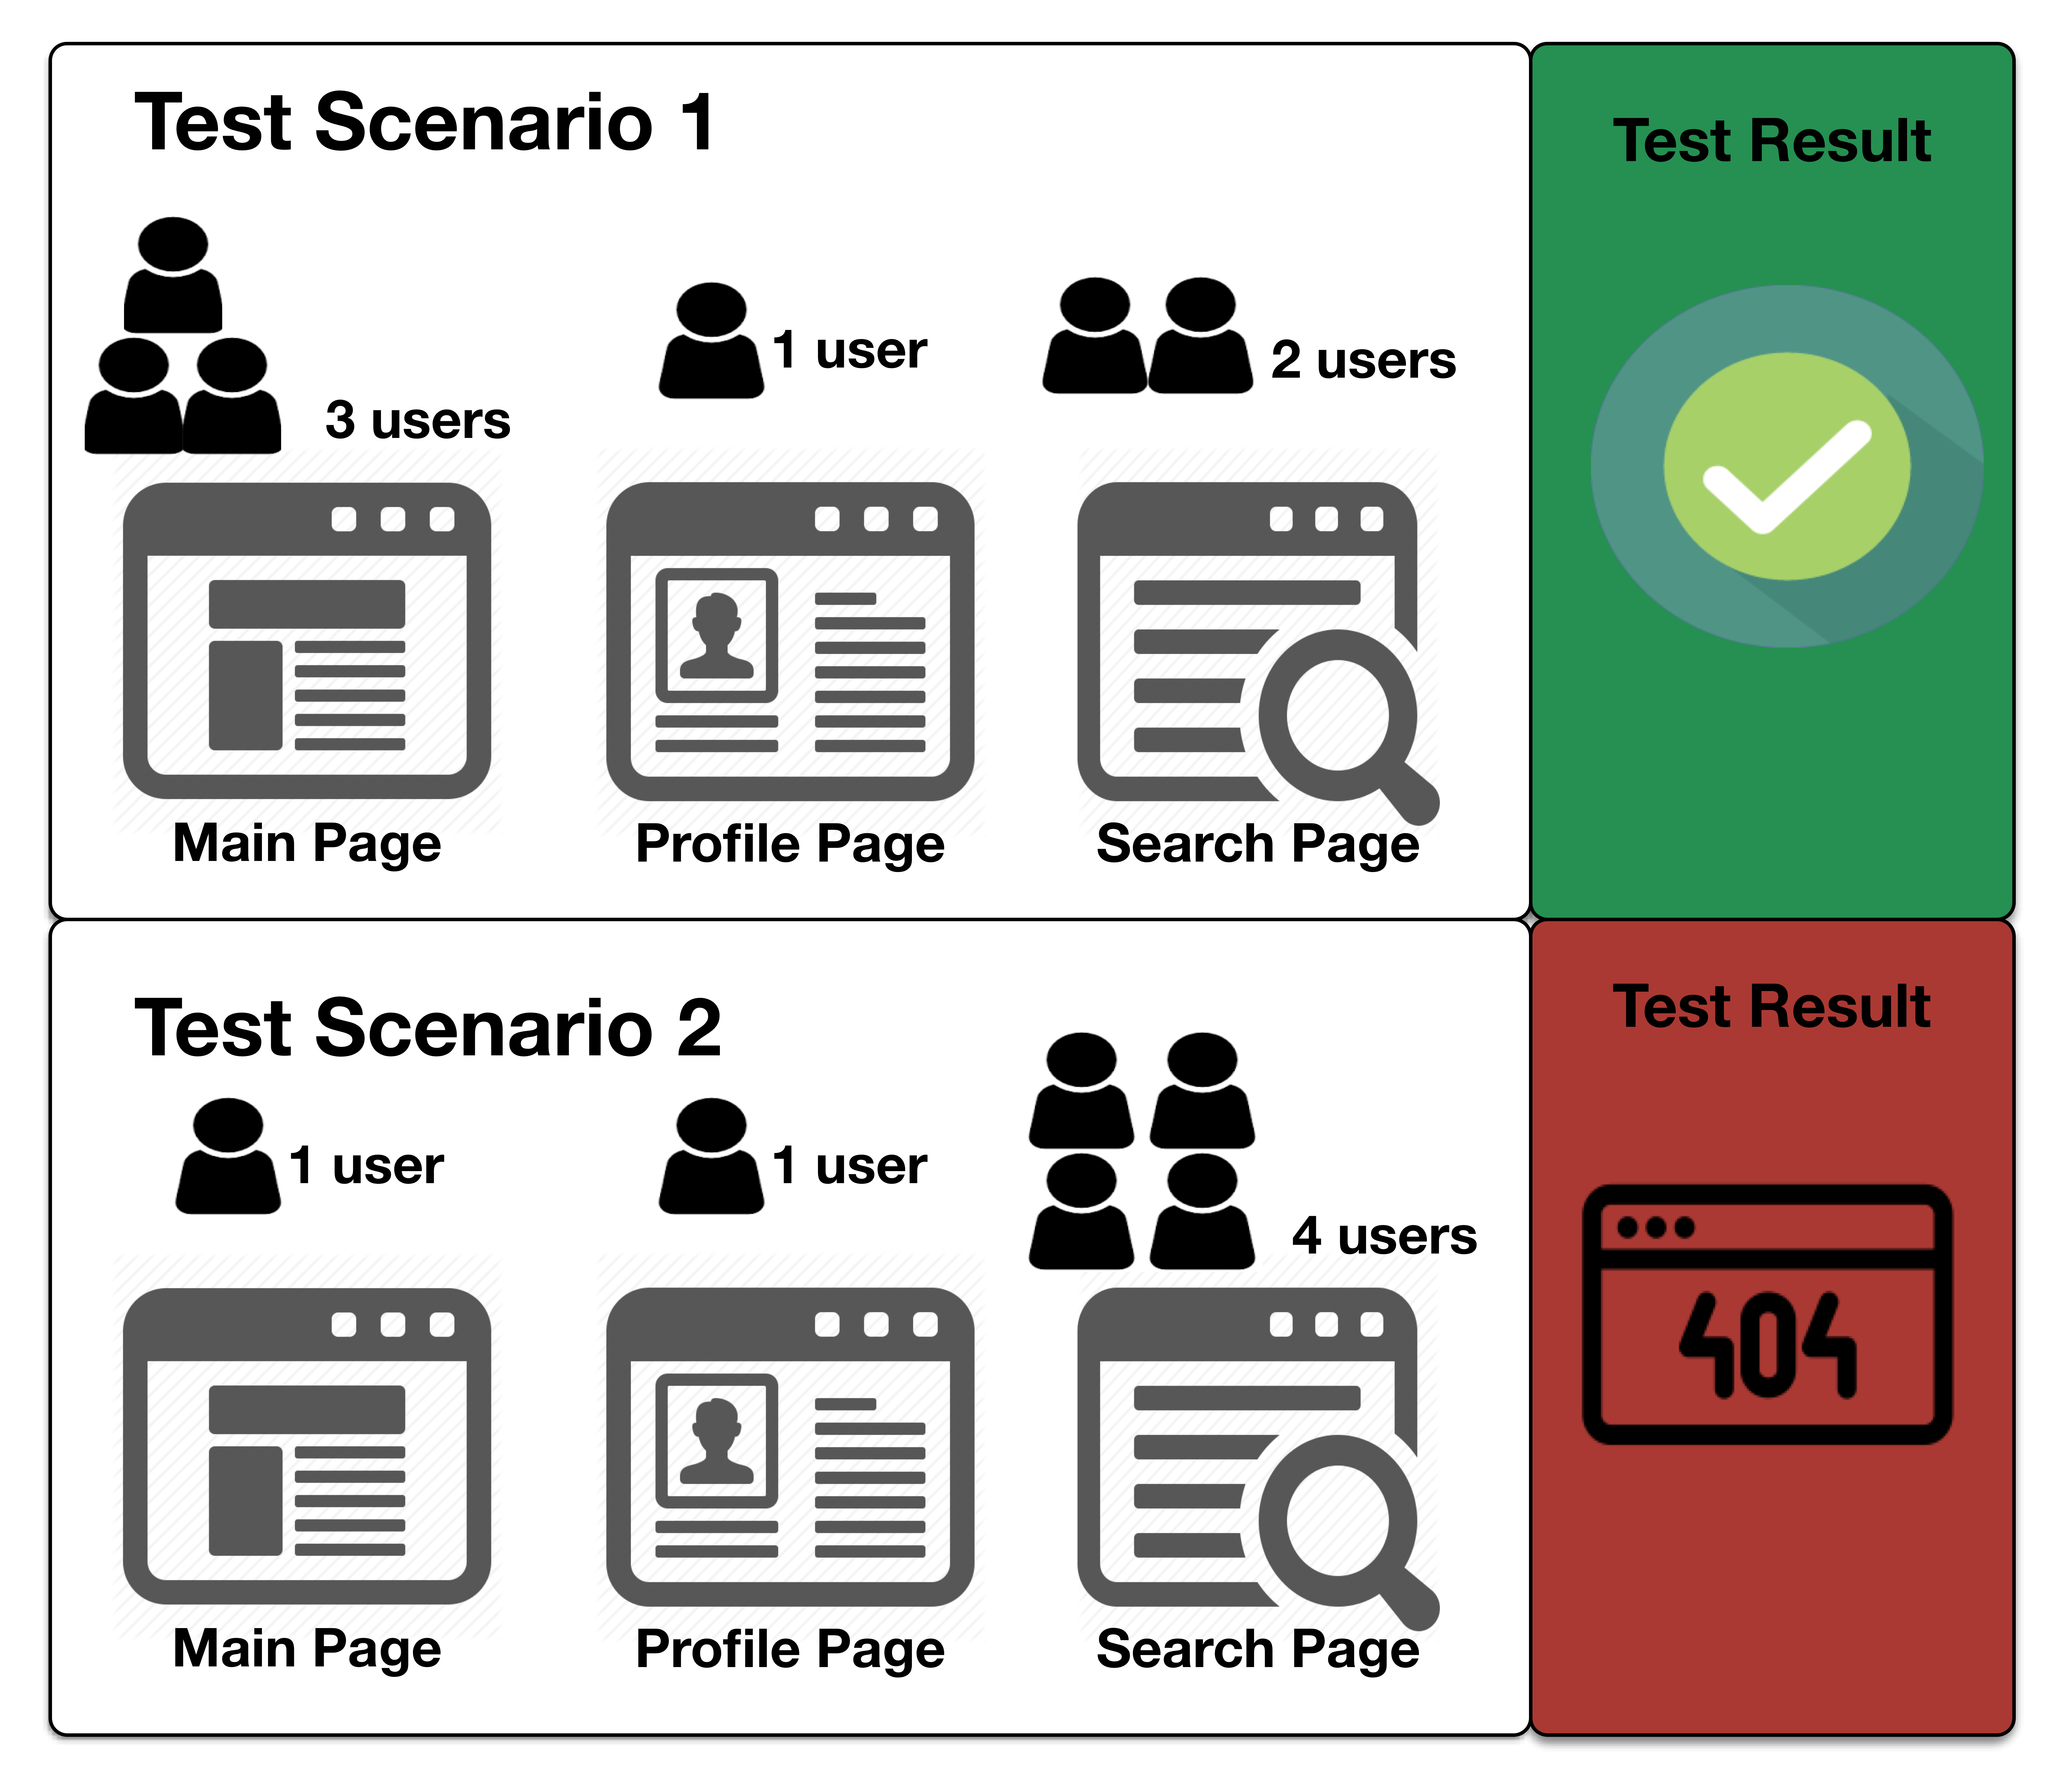
\includegraphics[width=0.4\textwidth]{./images/diagram.png}
\caption{Possible test scenarios for a hypothetical application}
\label{fig:example}
\end{figure}

A stress test usually lasts for several hours or even a few days and only tests a limited number of workloads. The major challenge is to find the workloads that expose a major number of errors and to discover the maximum number of users supported by an application under testing \cite{Barna2011}. 

Search-based testing is seen as a promising approach to verifying timing constraints \cite{Afzal2009a}. A common objective of a load search-based test is to find  scenarios that produce execution times that violate the specified timing constraints \cite{Sullivan}. 

This paper has two main goals:

\begin{itemize}
\item  To ascertain whether hybrid algorithms are superior to single metaheuristics when solving stress testing problem.
\item To improve the process of stress testing with a tool and a test model that evolves during its execution.
\end{itemize}




\begin{figure}[ht]
\centering
\includegraphics[width=0.25\textwidth]{./images/solution.png}
\caption{Illustrative example showing how IAdapter should be used}
\label{fig:solution}
\end{figure}


This paper proposes the use of a hybrid metaheuristic approach that combines genetic algorithms, simulated annealing, and tabu search algorithms in stress tests. A tool named IAdapter (www.iadapter.org, github.com/naubergois/newiadapter), a JMeter plugin for performing search-based load tests, was developed. Two experiments were conducted to validate the proposed approach. The first experiment was performed on an emulated component, and the second one was performed using an installed Moodle application. Fig. \ref{fig:solution} shows an example where IAdapter stress test automation finds two test scenarios. The first scenario presents a test that has an HTTP 500 error, and the second scenario presents a test that has a response time higher than 30 seconds. 

The remainder of the paper is organized as follows. Section 2 presents a brief introduction about load, performance, and stress tests. Section 3 presents concepts about the workload model. Section 4 presents concepts about search based tests. Section 5 presents concepts about metaheuristic algorithms.Section 6 presents concepts about hybrid metaheuristic algorithms. Section 7 discusses the related work. Section 8 presents the research-proposed approach. Section 9 presents the IAdapter tool. Section 10 shows the results of two experiments performed using the IAdapter plugin.  Conclusions and further work are presented in Section 11.




\section{Load, Performance and Stress Testing}

Load, performance, and stress testing are typically done to locate bottlenecks in a system, to support a performance-tuning effort, and to collect other performance-related indicators to help stakeholders get informed about the quality of the application being tested \cite{Sandler2004} \cite{Corporation2007}. 

The performance testing aims at verifying a specified system performance. This kind of test is executed by simulating hundreds of simultaneous users or more over a defined time interval \cite{DiLucca2006}. The purpose of this assessment is to demonstrate that the system reaches its performance objectives \cite{Sandler2004}. 


In a load testing, the system is evaluated at predefined load levels \cite{DiLucca2006}. The aim of this test is to determine whether the system can reach its performance targets for availability, concurrency, throughput, and response time. Load testing is the closest to real application use \cite{Molyneaux2009}.

The stress testing verifies the system behavior against heavy workloads \cite{Sandler2004}, which are executed to evaluate a system beyond its limits, validate system response in activity peaks, and verify whether the system is able to recover from these conditions. It differs from other kinds of testing in that the system is executed on or beyond its breakpoints, forcing the application or the supporting infrastructure to fail \cite{DiLucca2006} \cite{Molyneaux2009}.

The next subsections present details about the stress test process, automated stress test tools and the stress test results.

\subsection{Stress Test Process}

Contrary to functional testing, which has clear testing objectives, Stress testing objectives are not clear in the early development stages and are often defined later on a case-by-case basis. The Fig. \ref{fig:testprocess} shows a commom Load, Performance and Stress test process  \cite{Jiang2010}.

\begin{figure}[!ht]
\centering
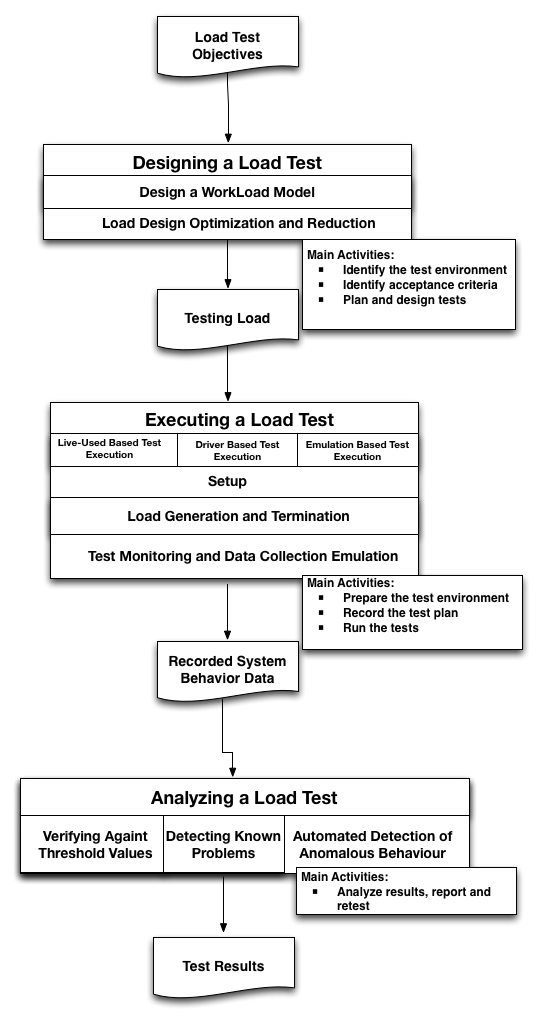
\includegraphics[width=0.5\textwidth]{./images/testprocess.png}
\caption{Load, Performance and Stress Test Process \cite{Jiang2010}\cite{Erinle2013}}
\label{fig:testprocess}
\end{figure}


The goal of the load design phase is to devise a load, which can uncover non-functional problems. Once the load is defined, the system under test executes the load and the system behavior under load is recorded. Load testing practitioners then analyze the system behavior to detect problems \cite{Jiang2010}. 

Once a proper load is designed, a load test is executed. The load test execution phase consists of the following three main aspects: (1) Setup, which includes system deployment and test execution setup; (2) Load Generation and Termination, which consists of generating the load; and (3) Test Monitoring and Data Collection, which includes recording the system behavior during execution\cite{Jiang2010}. 

The core activities in conducting an usual Load, Performance and Stress tests are \cite{Erinle2013}: 

\begin{itemize}
\item Identify the test environment: identify test and production environments and knowing the hardware, software, and network configurations helps derive an effective test plan and identify testing challenges from the outset.

\item Identify acceptance criteria: identify the response time, throughput, and resource utilization goals and constraints.

\item Plan and design tests:identify the test scenarios.In the context of testing, a scenario is a sequence of steps in an application. It can represent a use case or a business function such as searching a product catalog, adding an item to a shopping cart, or placing an order \cite{Corporation2007}.

\item Prepare the test environment: configure the test environment, tools, and resources necessary to conduct the planned test scenarios.

\item Record the test plan: record the planned test scenarios using a testing tool.

\item Run the tests: Once recorded, execute the test plans under light load and verify the correctness of the test scripts and output results.

\item Analyze results, report, and retest: examine the results of each successive run and identify areas of bottleneck that need addressing.  

\end{itemize}



\subsection{Automated Stress Test Tools}

Automated tools are needed to carry out serious load, stress, and performance testing. Sometimes, there is simply no practical way to provide reliable, repeatable performance tests without using some form of automation. The aim of any automated test tool is to simplify the testing process. Automated Test Tool  typically have the following components \cite{Molyneaux2009}:

\begin{itemize}
\item Scripting module: Enable recording of end-user activities in different middleware protocols;
\item Test management module: Allows the creation of test scenarios;
\item Load injectors: Generate the load with multiple workstations or servers;
\item Analysis module: Provides the ability to analyse the data collected by each test interation.
\end{itemize}

Apache JMeter is a free open source stress testing tool.  It has a large user base and offers lots of plugins to aid testing. JMeter is a desktop application designed to test and measure the performance and functional behavior of applications. The application it's purely Java-based and is highly extensible through a provided API (Application Programming Interface). JMeter works by acting as the client of a client/server application. JMeter allows multiple concurrent users to be simulated on the application \cite{Halili2008} \cite{Erinle2013}. JMeter has components organized  in a hierarchical manner. The Test Plan is the main component in a JMeter script. A typical test plan will consist of one or more Thread Groups, logic controllers, listeners, timers, assertions, and configuration elements:

\begin{itemize}
\item Thread Group: Test management module responsible to simulate the users used in a test. All elements of a test plan must be under a thread group.
\item Listeners: Analysis module responsible to provide access to the information gathered by JMeter about the test cases .
\item Samplers: Load injectors module responsible to send requests to a server, while Logical Controllers let you customize its logic.
\item Timers: allow JMeter to delay between each request.
\item Assertions: test if the application under test it is returning the correct results.
\item Configuration Elements: configure detais about the request protocol and test elements.
\end{itemize}


\subsection{Stress Test Results}

The system behavior recorded during the test execution phase needs to be analyzed to determine if there are any load-related functional or non-functional problems \cite{Jiang2010}.

There can be many formats of system behavior like resource usage data or end-to-end response time, which is recorded as response time for each individual request. These types of data need to be processed before comparing against threshold values.A proper data summarization technique is needed to describe these many data instances into one number. Some researchers advocate that the 90-percentile response time is a better measurement than the average/medium response time, as the former accounts for most of the peaks, while eliminating the outliers \cite{Jiang2010}.


\section{WorkLoad Model}

Load, performance, or stress testing projects should start with the development of a model for user workload that an application receives. This should take into consideration various performance aspects of the application and the infrastructure that a given workload will impact. A workload is a key component of such a model \cite{Molyneaux2009}.

The term workload represents the size of the demand that will be imposed on the application under test in an execution. The metric  used for measure a workload is dependent on the application domain, such as the length of the video in a transcoding application for multimedia files or the size of the input files in a file compression application \cite{Feitelson2013} \cite{Molyneaux2009} \cite{Goncalves2014}. 

Workload is also defined by the load distribution between the identified transactions at a given time. Workload helps researchers study the system behavior identified in several load models. A workload model can be designed to verify the predictability, repeatability, and scalability of a system \cite{Feitelson2013} \cite{Molyneaux2009}.


Workload modeling is the attempt to create a simple and generic model that can then be used to generate synthetic workloads. The goal is typically to be able to create workloads that can be used in performance evaluation studies. Sometimes, the synthetic workload is supposed to be similar to those that occur in practice in real systems \cite{Feitelson2013} \cite{Molyneaux2009}.

There are two kinds of workload models: descriptive and generative. The main difference between the two is that descriptive models just try to mimic the phenomena observed in the workload, whereas generative models try to emulate the process that generated the workload in the first place \cite{DiLucca2006}. 

In descriptive models, one finds different levels of abstraction on the one hand and different levels of fidelity to the original data on the other hand. The most strictly faithful models try to mimic the data directly using the statistical distribution of the data. The most common strategy used in descriptive modeling is to create a statistical model of an observed workload (Fig. \ref{fig:descriptivemodel}). This model is applied to all the workload attributes, e.g., computation, memory usage, I/O behavior, communication, etc. \cite{DiLucca2006}. Fig. \ref{fig:descriptivemodel} shows a simplified workflow of a descriptive model. The workflow has six phases. In the first phase, the user uses the system in the production environment. In the second phase, the tester collects the user's data, such as logs, clicks, and preferences, from the system. The third phase consists in developing a model designed to emulate the user's behavior. The fourth phase is made up of the execution of the test, emulation of the user's behavior, and log gathering.



\begin{figure}[H]
\centering
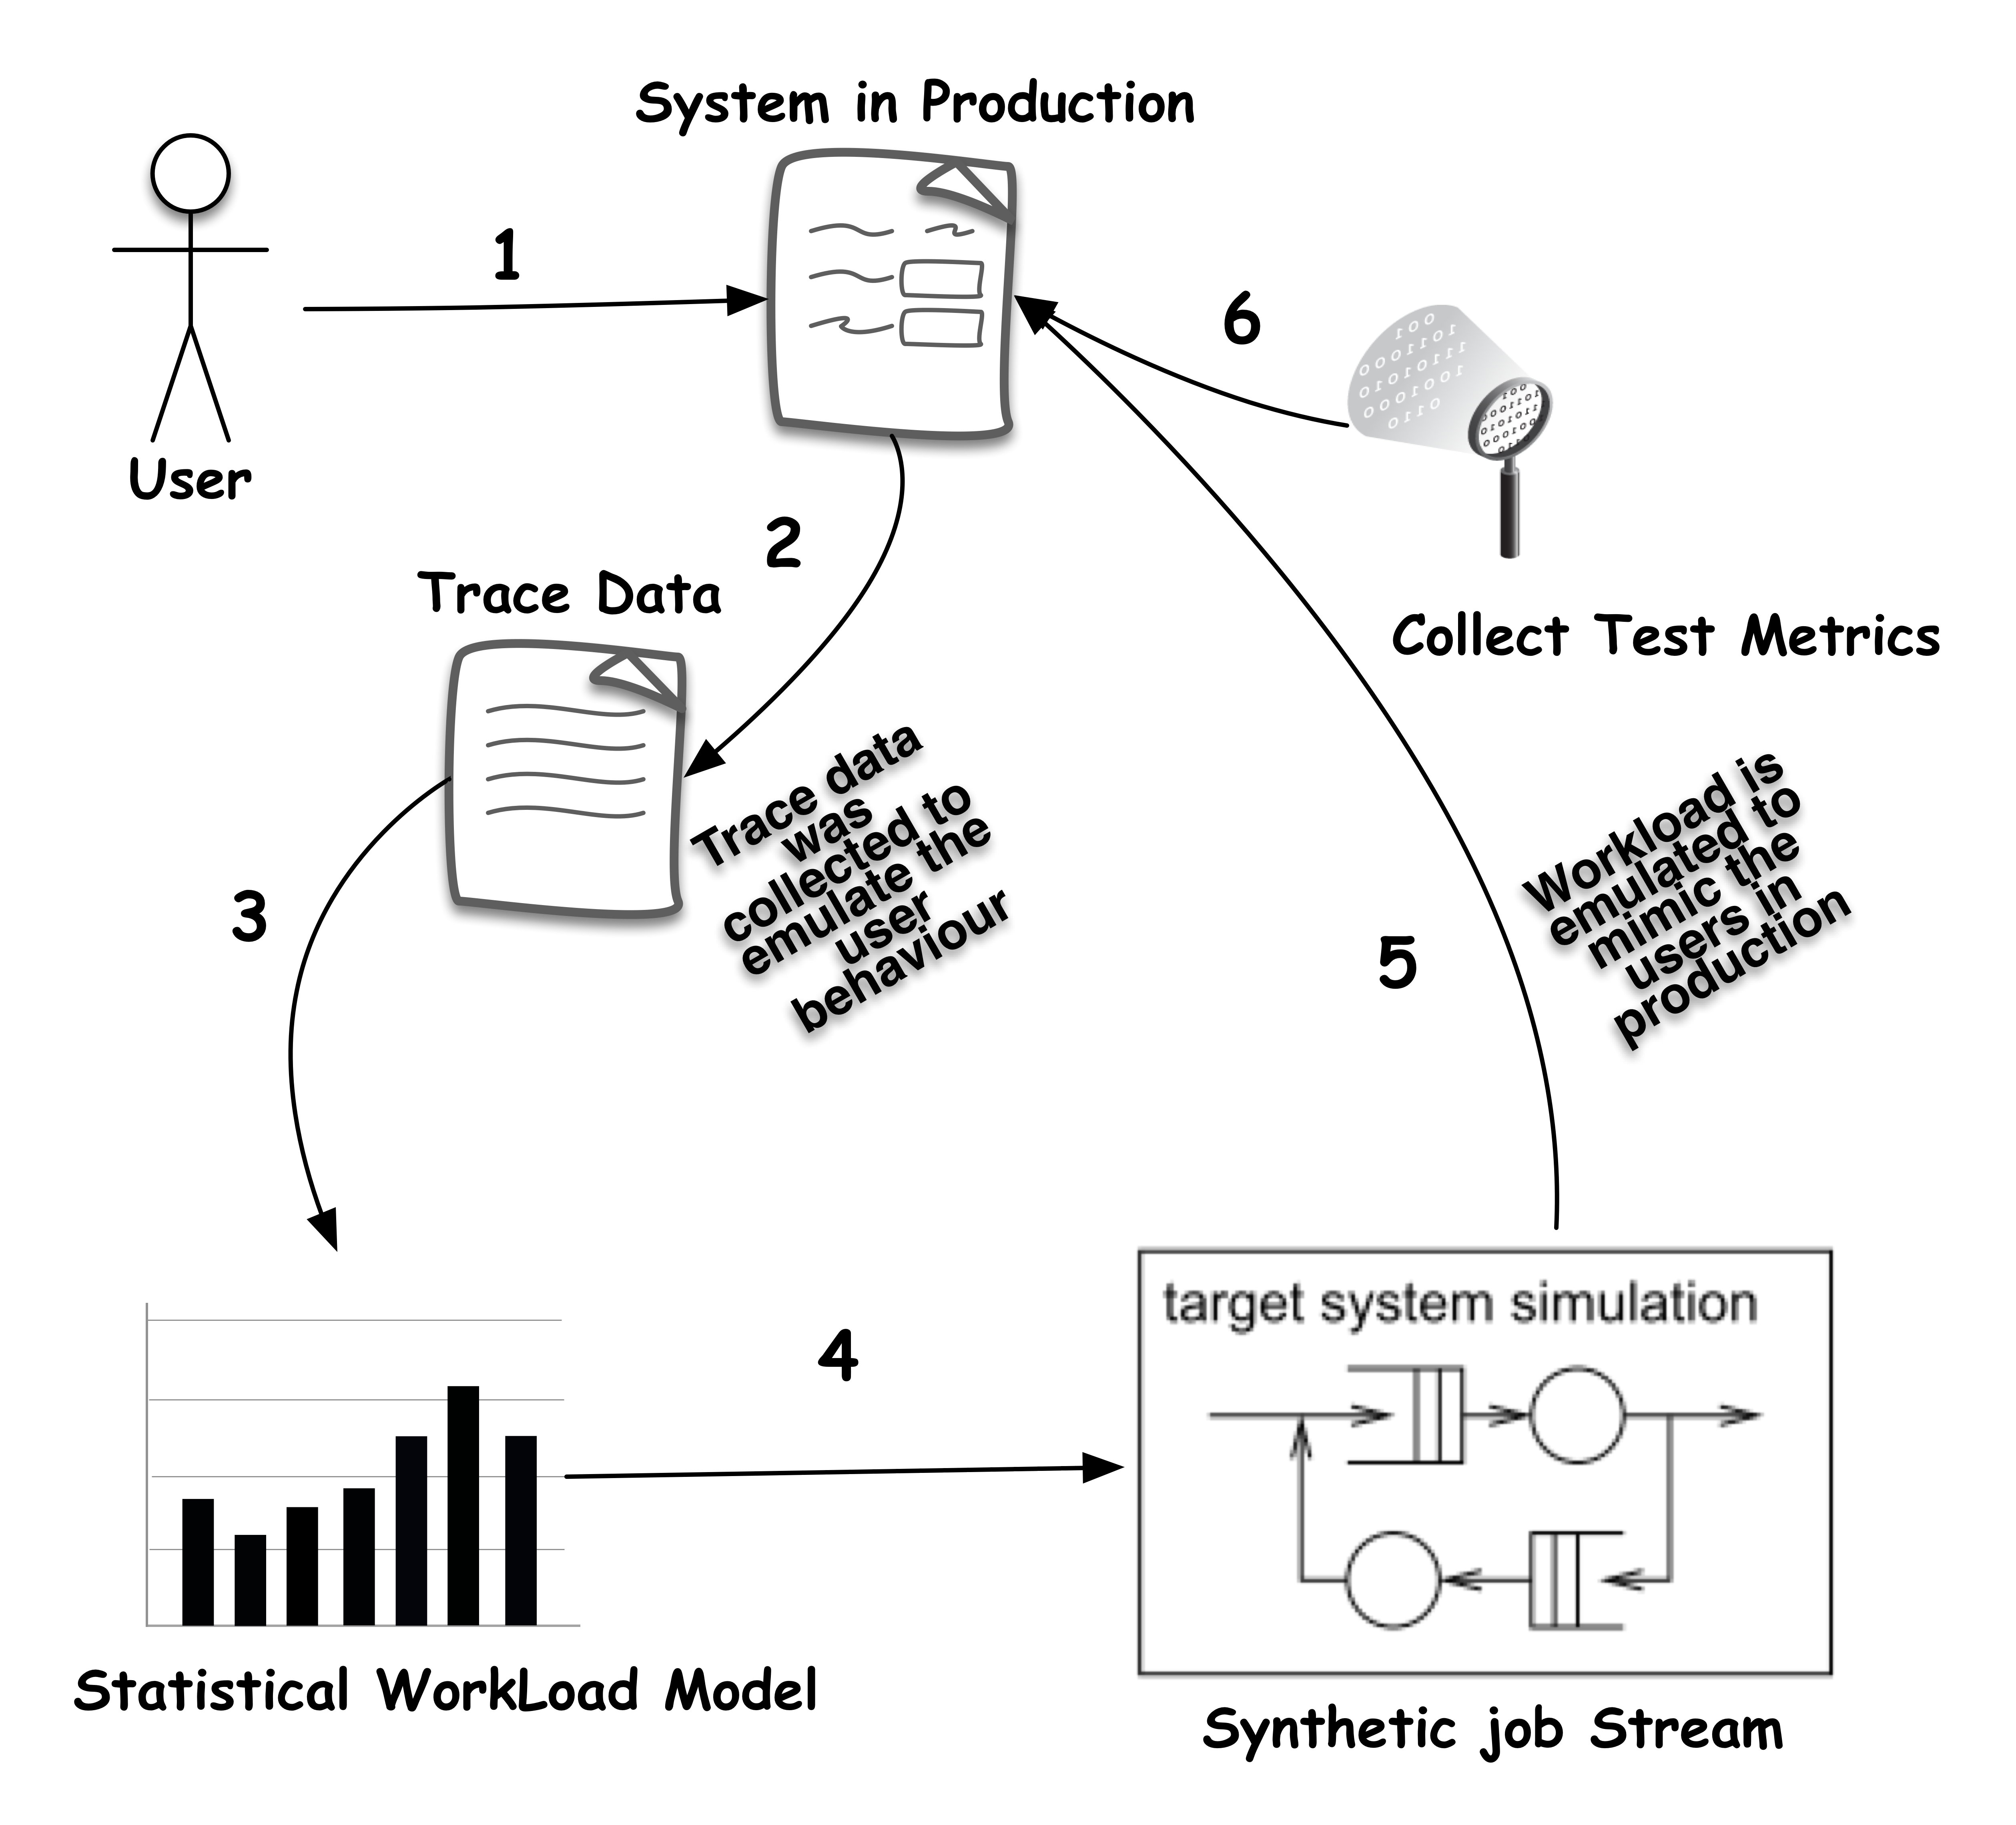
\includegraphics[width=0.4\textwidth]{./images/workloadmodel1300dpi.png}
\caption{Workload modeling based on statistical data \cite{DiLucca2006}}
\label{fig:descriptivemodel}
\end{figure}

Generative models are indirect in the sense that they do not model the statistical distributions. Instead, they describe how users will behave when they generate the workload. An important benefit of the generative approach is that it facilitates manipulations of the workload. It is often desirable to be able to change the workload conditions as part of the evaluation. Descriptive models do not offer any option regarding how to do so. With the generative models, however, we can modify the workload-generation process to fit the desired conditions \cite{DiLucca2006}. The difference between the workflows of the descriptive and the generative models is that user behavior is not collected from logs, but simulated from a model that can receive feedback from the test execution (Fig. \ref{fig:generativemodel}).

\begin{figure}[H]
\centering
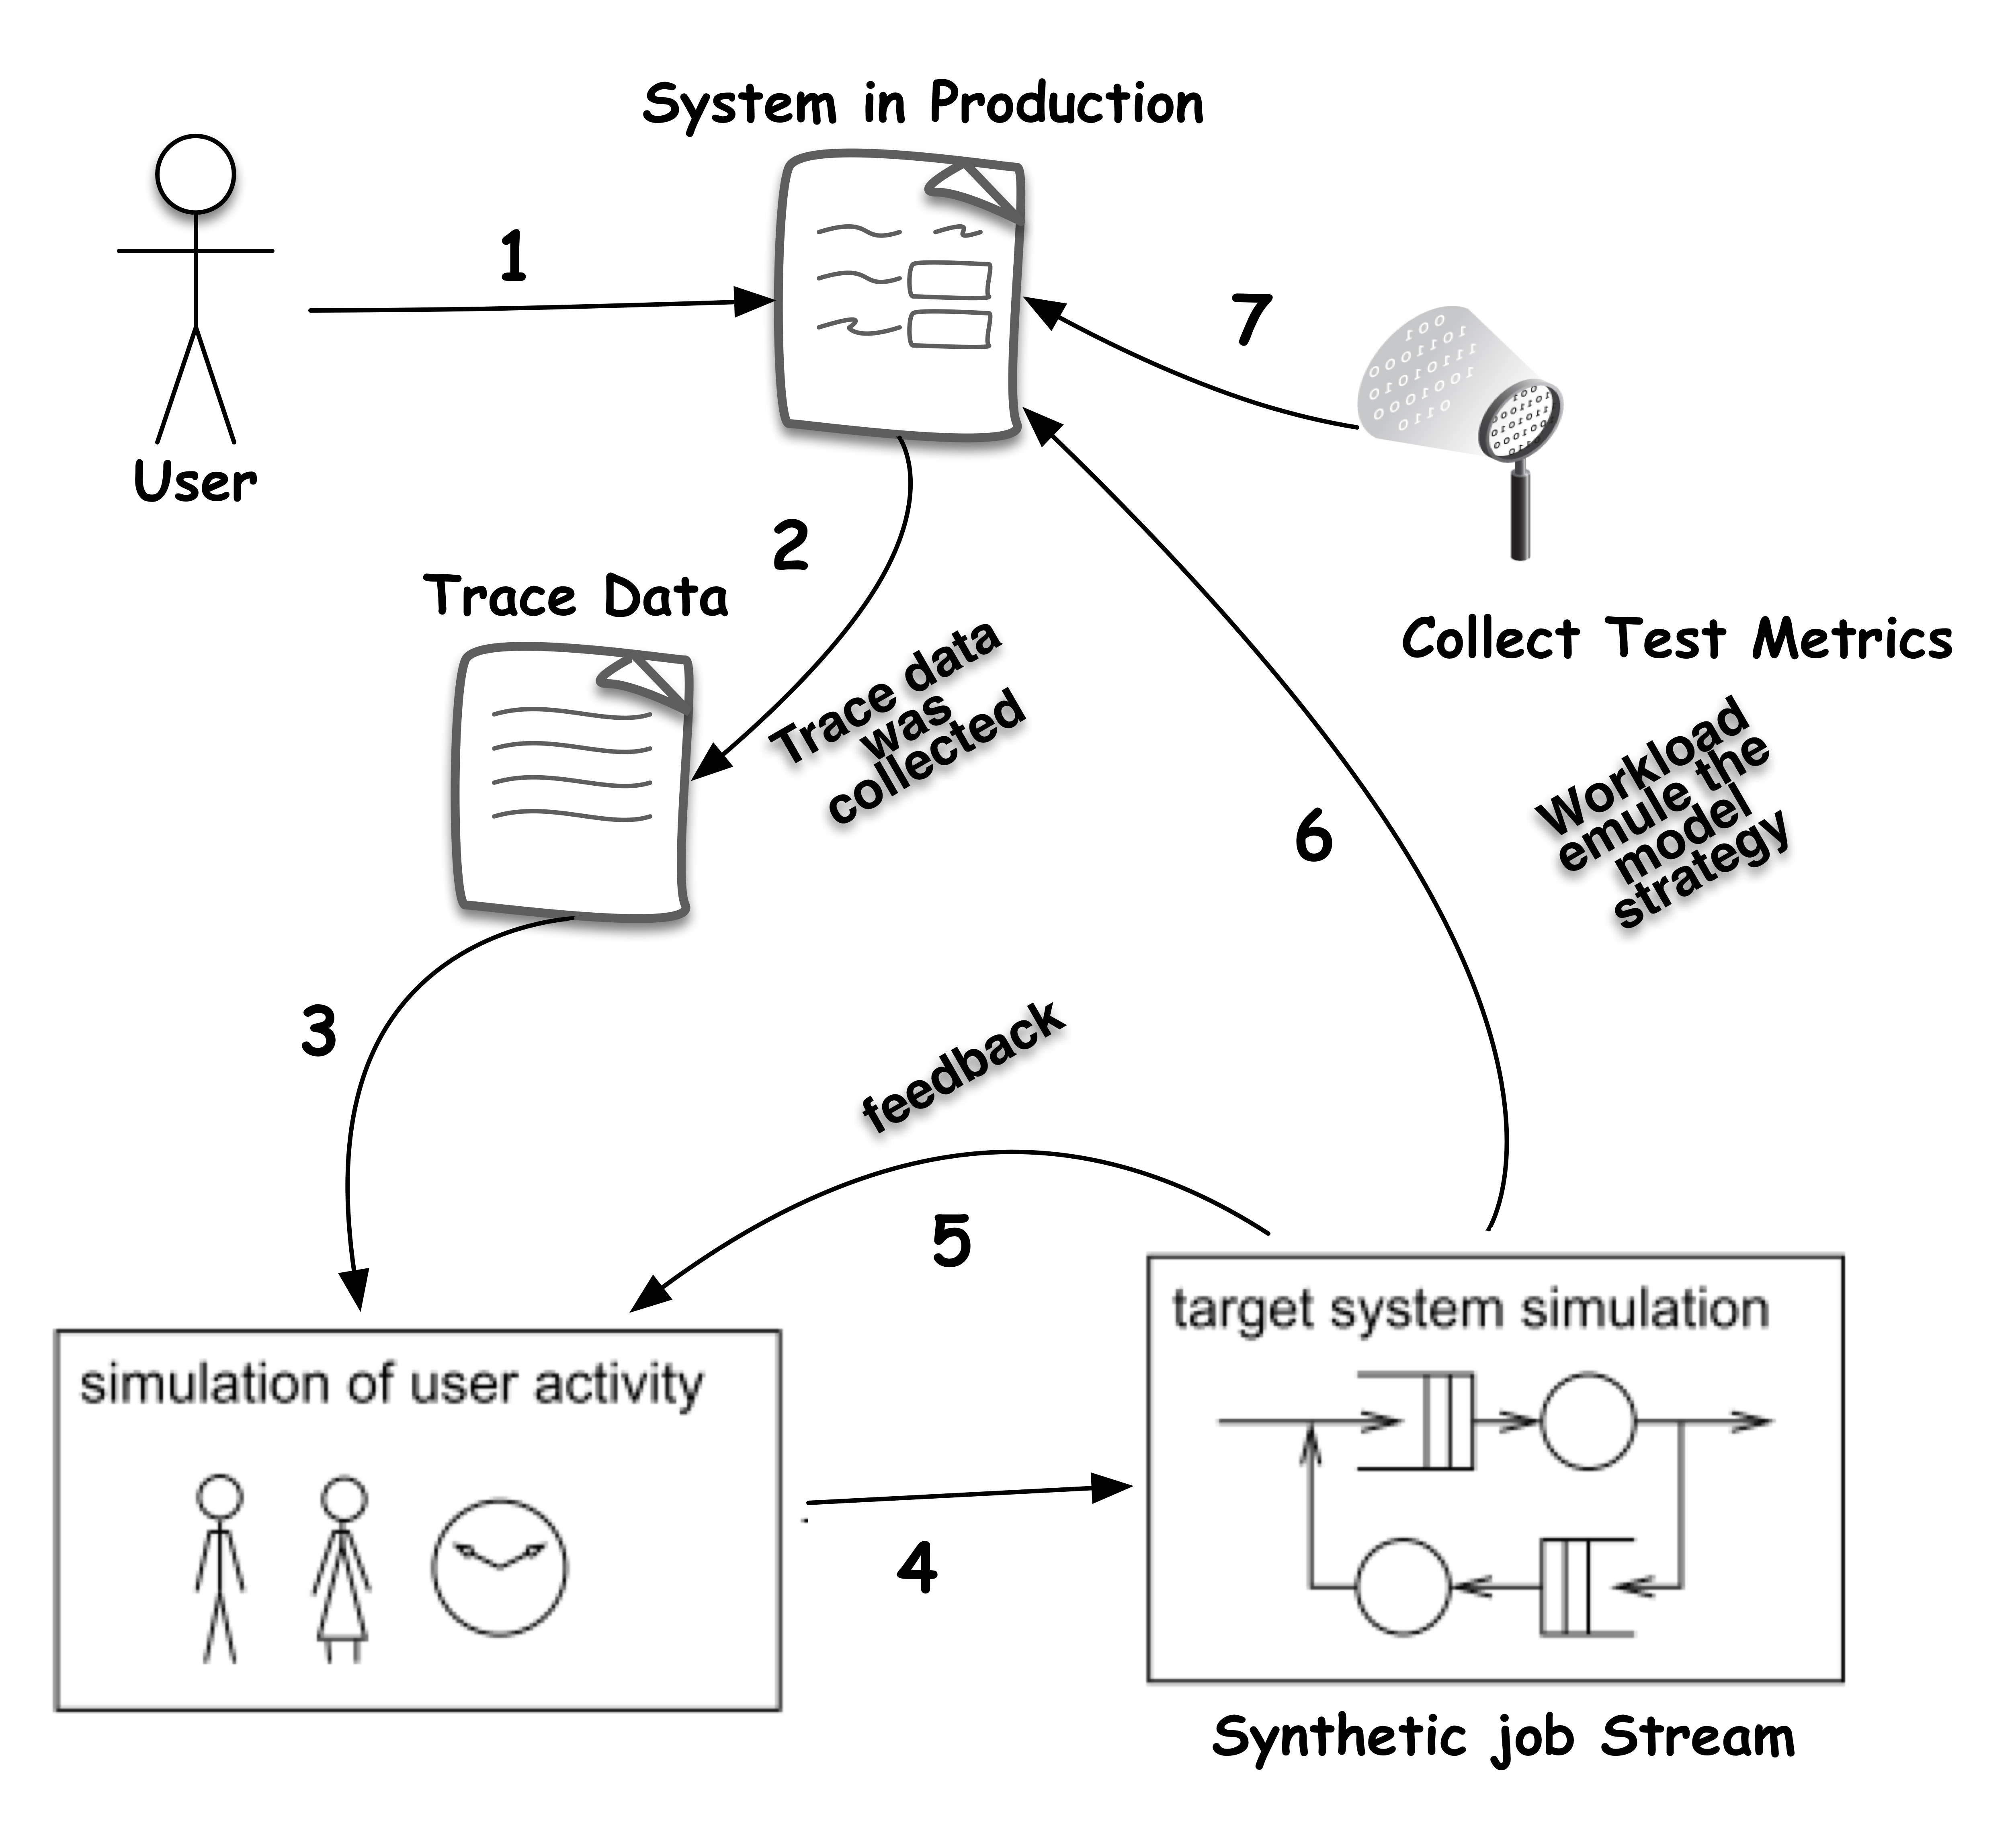
\includegraphics[width=0.4\textwidth]{./images/workloadmodel2300dpi.png}
\caption{Workload modeling based on the generative model \cite{DiLucca2006}}
\label{fig:generativemodel}
\end{figure}

Both load model have their advantages and disadvantages. In general, loads resulting from realistic-load based design techniques (Descriptive models) can be used to detect both functional and non-functional problems. However, the test durations are usually longer and the test analysis is more difficult. Loads resulting from fault-inducing load design techniques (Generative models) take less time to uncover potential functional and non-functional problems, the resulting loads usually only cover a small portion of the testing objectives \cite{Jiang2010}. The presented research work uses a generative model.

\section{Search Based Tests}

Search-based software engineering (SBSE) is the application of optimization techniques in solving software engineering problems. The applicability of optimization techniques in solving software engineering problems is suitable as these problems frequently encounter competing constraints and require near optimal solutions \cite{Afzal2009a} \cite{Harman2015}. 


Search Based Software Testing (SBST) is the sub-area of Search Based Software Engineering concerned with software testing. Search-based software testing is the application of metaheuristic search techniques to generate software tests. SBSE uses computational search techniques to tackle software engineering problems, typified by large complex search spaces. SBSE derives test inputs for a software system with the goal of improving various criteria. The test adequacy criterion is transformed into a fitness function and a set of solutions in the search space are evaluated with respect to the fitness function using a metaheuristic search technique \cite{Afzal2009a} \cite{Aleti2016} \cite{Harman2015}.


Figure \ref{fig:sbsesbst}  shows the growth in papers published on SBST and SBSE. The data is taken from the SBSE repository (\url{http://crestweb.cs.ucl.ac.uk/resources/sbse_repository/}). 
The aim of the SBSE repository is to contain every SBSE paper. Although no repository can guarantee 100\% precision and recall, the SBSE repository has proved sufficiently usable that it has formed the basis of several other detailed analyses of the literature \cite{Harman2015}. 


\begin{figure}[h]
\centering
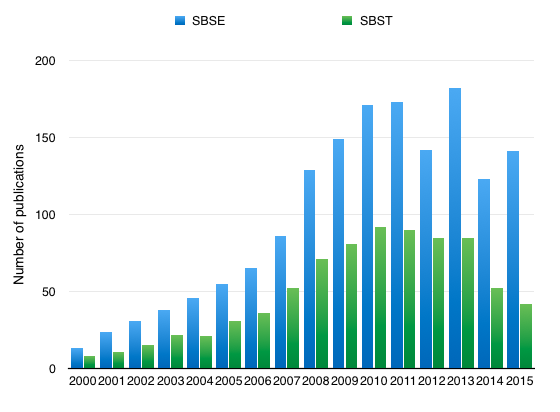
\includegraphics[width=0.5\textwidth]{./images/publications1.png}
\caption{Number of publications in SBSE and SBST by Year. Data comes from the Harman et al., Afzal et al. and the SBSE repository  \cite{Afzal2009a} \cite{Harman2015}}
\label{fig:sbsesbst}
\end{figure}


SBST has made many achievements, and demonstrated its wide applicability and increasing uptake. Nevertheless, there are pressing open problems and challenges that need more attention like to extend SBST to test non-functional properties, a topic that remains relatively under-explored, compared to structural testing. The Fig. \ref{fig:nonfunctional} shows the non-funtional SBST by year \cite{Aleti2016} \cite{Harman2015}. 

\begin{figure}[h]
\centering
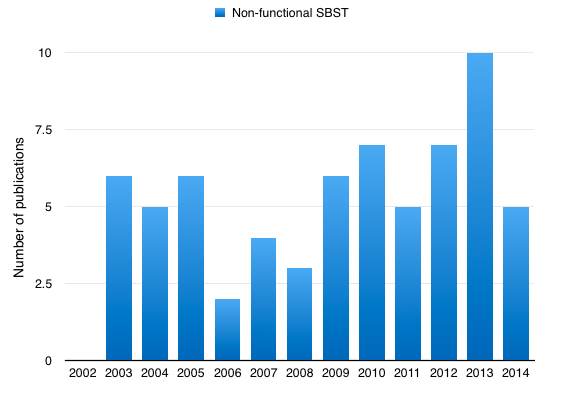
\includegraphics[width=0.5\textwidth]{./images/nonfunctional.png}
\caption{Number of publications in non-functional SBST by Year. Data comes from the Harman et al., Afzal et al. and the SBSE repository  \cite{Afzal2009a} \cite{Harman2015} }
\label{fig:nonfunctional}
\end{figure}

There are many kinds of non-functional search based tests  \cite{Afzal2009a}:

\begin{itemize}
\item Execution time: The application of evolutionary algorithms to find the best and worst case execution times (BCET, WCET).
\item Quality of service: uses metaheuristic search techniques to search violations of service level agreements (SLAs).
\item Security: apply a variety of metaheuristic search techniques  to detect security vulnerabilities like detecting buffer overflows.
\item Usability: concerned with construction of covering array which is a combinatorial object.
\item Safety: Safety testing is an important component of the testing strategy of safety critical systems where the systems are required to meet safety constraints.
\end{itemize}

A variety of metaheuristic search techniques are found to be applicable for non-functional testing including simulated annealing, tabu search, genetic algorithms, ant colony methods, grammatical evolution, genetic programming and swarm intelligence methods. The Table \ref{table:metaheuriscbysbst} shows the number of papers by metaheuristc and kind of SBST. The data of the table was extracted from Afzal et al. \cite{Afzal2009a}.

\begin{table}[H]
\centering
\caption{Metaheuristic by Kind of SBST. Data comes from  Afzal et al. \cite{Afzal2009a}}
\label{table:metaheuriscbysbst}
\begin{tabular}{|l|l|l|}
\hline
Metaheuristc                       & Number of Papers & Kind of SBST                                            \\
\hline
Genetic Algorithm(GA) and Simulated Annealing(SA)                          & 1                & Safety                                                  \\
\hline
SA                                 & 4                & Safety, Usability and Execution Time                    \\
\hline
Grammatical Evolution              & 1                & Security                                                \\
\hline
Linear Genetic Programming         & 2                & Security                                                \\
\hline
GA and Particle swarm optimization & 1                & Security                                                \\
\hline
Tabu Search (TS), SA and GA                      & 1                & Usability                                               \\
\hline
SA and hill climbing               & 1                & Usability                                               \\
\hline
TS                                 & 1                & Usability                                               \\
\hline
Hill climbing, SA and TS           & 1                & Usability                                               \\
\hline
Ant colony and GA                  & 1                & Usability                                               \\
\hline
GA                                 & 16               & Safety, Security, QoS and Execution Time \\
\hline
\end{tabular}
\end{table}

\section{Metaheuristics}

In the computer science, the term metaheuristic is accepted for general techniques which are not specific to a particular problem. A metaheuristic is formally defined as an iterative generation process which guides a subordinate heuristic by combining intelligently different concepts for exploring and exploiting the search space \cite{raidl2010metaheuristic}. 

Metaheuristics are strategies that guide the search process to efficiently explore the search space in order to find optimal solutions. Metaheuristic algorithms are approximate and usually non-deterministic and sometimes incorporate mechanisms to avoid getting trapped in confined areas of the search space. There are different ways to classify and describe metaheuristic algorithm \cite{Blum2003}:

\begin{itemize}
\item Nature-inspired vs. non-nature inspired. There are nature-inspired algorithms, like Genetic Algorithms and Ant Algorithms, and non nature-inspired ones such as Tabu Search and Iterated Local Search. 

\item Population-based vs. single point search. Algorithms working on single solutions are called trajectory methods, like Tabu Search, Iterated Local Search and Variable Neighborhood Search. They all share the property of describing a trajectory in the search space during the search process. Population-based metaheuristics perform search processes which describe the evolution of a set of points in the search space.

\item One vs. various neighborhood structures. Most metaheuristic algorithms work on one single neighborhood structure. In other words, the fitness landscape topology does not change in the course of the algorithm. Other metaheuristics, such as Variable Neighborhood Search (VNS), use a set of neighborhood structures which gives the possibility to diversify the search by swapping between different fitness
landscapes.


\end{itemize}

Trajectory methods are characterized by a trajectory in the search space. Two common trajectory methods are Simulated Annealing and Tabu Search.

Simulated Annealing (SA) is a randomized algorithm that tries to avoid being trapped in local optimum solution by assigning probabilities to deteriorating moves. The SA procedure is inspired from the annealing process of solids. SA is based on a physical
process in metallurgy discipline or solid matter physics. Annealing is the process of obtaining low energy states of a solid in heat treatment \cite{Jaziri2008}. 

The algorithmic framework of SA is described in Alg. \ref{sa}.  The algorithm starts by generating an initial solution in function \textit{GenerateInitialSolution()}. The initial temperature value is determined in function \textit{SetInitialTemperature()} such that the probability for an uphill move is quite high at the start of the algorithm. At each iteration a solution $\mbox{s}_1$ is randomly chosen in function \textit{PickNeighborAtRandom(N(s))}. If \textit{$\mbox{s}_1$} is better than \textit{s}, then \textit{$\mbox{s}_1$} is accepted as new current solution. Else, if the move from \textit{s} to \textit{$\mbox{s}_1$} is an uphill move, \textit{$\mbox{s}_1$}  is accepted with a probability which is a function of a temperature parameter \textit{Tk} and \textit{s} \cite{raidl2010metaheuristic}. 

\begin{algorithm}[H]
  \caption{Simulated Annealing Algorithm}\label{sa}
  \begin{algorithmic}[1]
    
    \State $s\gets GenerateInitialSolution()$
    \State $k\gets 0 $
    \State $Tk\gets SetInitialTemperature()$
    \While{termination conditions not met }
    \State $\mbox{s}_1\gets PickNeighborAtRandom(N (s))$
    \If{$(f(\mbox{s}_1)<f(s))$}
    \State $s\gets\mbox{s}_1$
    \Else $\;$ Accept $\mbox{s}_1$ as new solution with probability p($\mbox{s}_1|$Tk,s) 
    \EndIf
    \State $K\gets K+1$
    \State $Tk\gets AdaptTemperature()$
    \EndWhile
      
  \end{algorithmic}
\end{algorithm}


Tabu Search is a metaheuristic that guides a local heuristic search procedure to explore the solution space beyond local optimal and search with short term memory to avoid cycles. Tabu Search uses a  tabu list to keep track of the last  moves, and don’t allow going back to these \cite{Glover1986}.

The algorithmic framework of Tabu Search is described in Alg. \ref{tsa}.  The algorithm starts by generating an initial solution in function \textit{GenerateInitialSolution()} and the tabu lists are initialized as empty lists in function \textit{InitializeTabuLists($\mbox{TL}_1$,...,$\mbox{TL}_r$)}. For performing a move, the algorithm first determines those solutions from the neighborhood \textit{N(s)} of the current solution \textit{s} that contain solution features currently to be found in the tabu lists. They are excluded from the neighborhood, resulting in a restricted set of neighbors \textit{$\mbox{N}_a(s)$}. At each iteration the best solution \textit{$\mbox{s}_1$} from \textit{$\mbox{N}_a(s)$} is chosen as the new current solution. Furthermore, in procedure \textit{UpdateTabuLists($\mbox{TL}_1$,...,$\mbox{TL}_r$,s,$\mbox{s}_1$)} the corresponding features of this solution are added to the tabu lists.


\begin{algorithm}[H]
  \caption{Tabu Search Algorithm}\label{tsa}
  \begin{algorithmic}[2]
    
    \State $s\gets GenerateInitialSolution()$
    \State InitializeTabuLists($\mbox{TL}_1$,...,$\mbox{TL}_r$)
    \While{termination conditions not met }
    \State $\mbox{N}_a(s)\gets$ $\{\mbox{s}_1 \in N(s) |\mbox{s}_1$ does not violate a tabu condition, or it satisfies at least one aspiration condition $\}$ 
    \State $\mbox{s}_1\gets argmin\{f(\mbox{s}_2)|\mbox{s}_2 \in \mbox{N}_a(s) \}$
    \State UpdateTabuLists($\mbox{TL}_1$,...,$\mbox{TL}_r$,s,$\mbox{s}_1$)
    \State $s\gets \mbox{s}_1$
    \EndWhile
      
  \end{algorithmic}
\end{algorithm}

Population-based metaheuristics (P-metaheuristics) could be viewed as an iterative improvement in a population of solutions. First, the population is initialized. Then, a new population of solutions is generated. Finally, this new population is integrated into the current one using some selection procedures. The search process is stopped when a stopping criterion is satisfied. Algorithms such as Genetic algorithms (GA), scatter search (SS), estimation of distribution algorithms (EDAs), particle swarm optimization (PSO), bee colony (BC), and artificial immune systems (AISs) belong to this class of metaheuristics \cite{talbi2009metaheuristics}. 

Algorithm \ref{gna} shows the basic structure of GA algorithms. In this algorithm, P denotes the population of individuals. A population of offspring is generated by the application of recombination and mutation operators and the individuals for the next population are selected from the union of the old population and the offspring population \cite{raidl2010metaheuristic}.


\begin{algorithm}[H]
  \caption{Genetic Algorithm}\label{gna}
  \begin{algorithmic}[3]
    
    \State $s\gets GenerateInitialSolution()$
    \State Evaluate(P)
    \While{termination conditions not met }
    \State $\mbox{P}_1\gets$ $Recombine(P)$
    \State $\mbox{P}_2\gets$ $Mutate(\mbox{P}_1)$ 
    \State $Evaluate(\mbox{P}_2)$
    \State $P\gets Select(\mbox{P}_2,P)$
    \EndWhile
      
  \end{algorithmic}
\end{algorithm}


\section{Hybrid  Metaheuristics}

A combination of one metaheuristic with components from other metaheuristics is called a hybrid metaheuristic. The concept of hybrid metaheuristics has been commonly accepted only in recent years, even if the idea of combining different metaheuristic strategies and algorithms dates back to the 1980s. Today, we can observe a generalized common agreement on the advantage of combining components from different search techniques and the tendency of designing hybrid techniques is widespread in the fields of operations research and artificial intelligence \cite{raidl2010metaheuristic}. 


There are two main categories of metaheuristic combinations: collaborative combinations and integrative combinations. These are presented in Fig. \ref{fig:metaheuristc} \cite{Raidl2006}.

\begin{figure}[H]
\centering
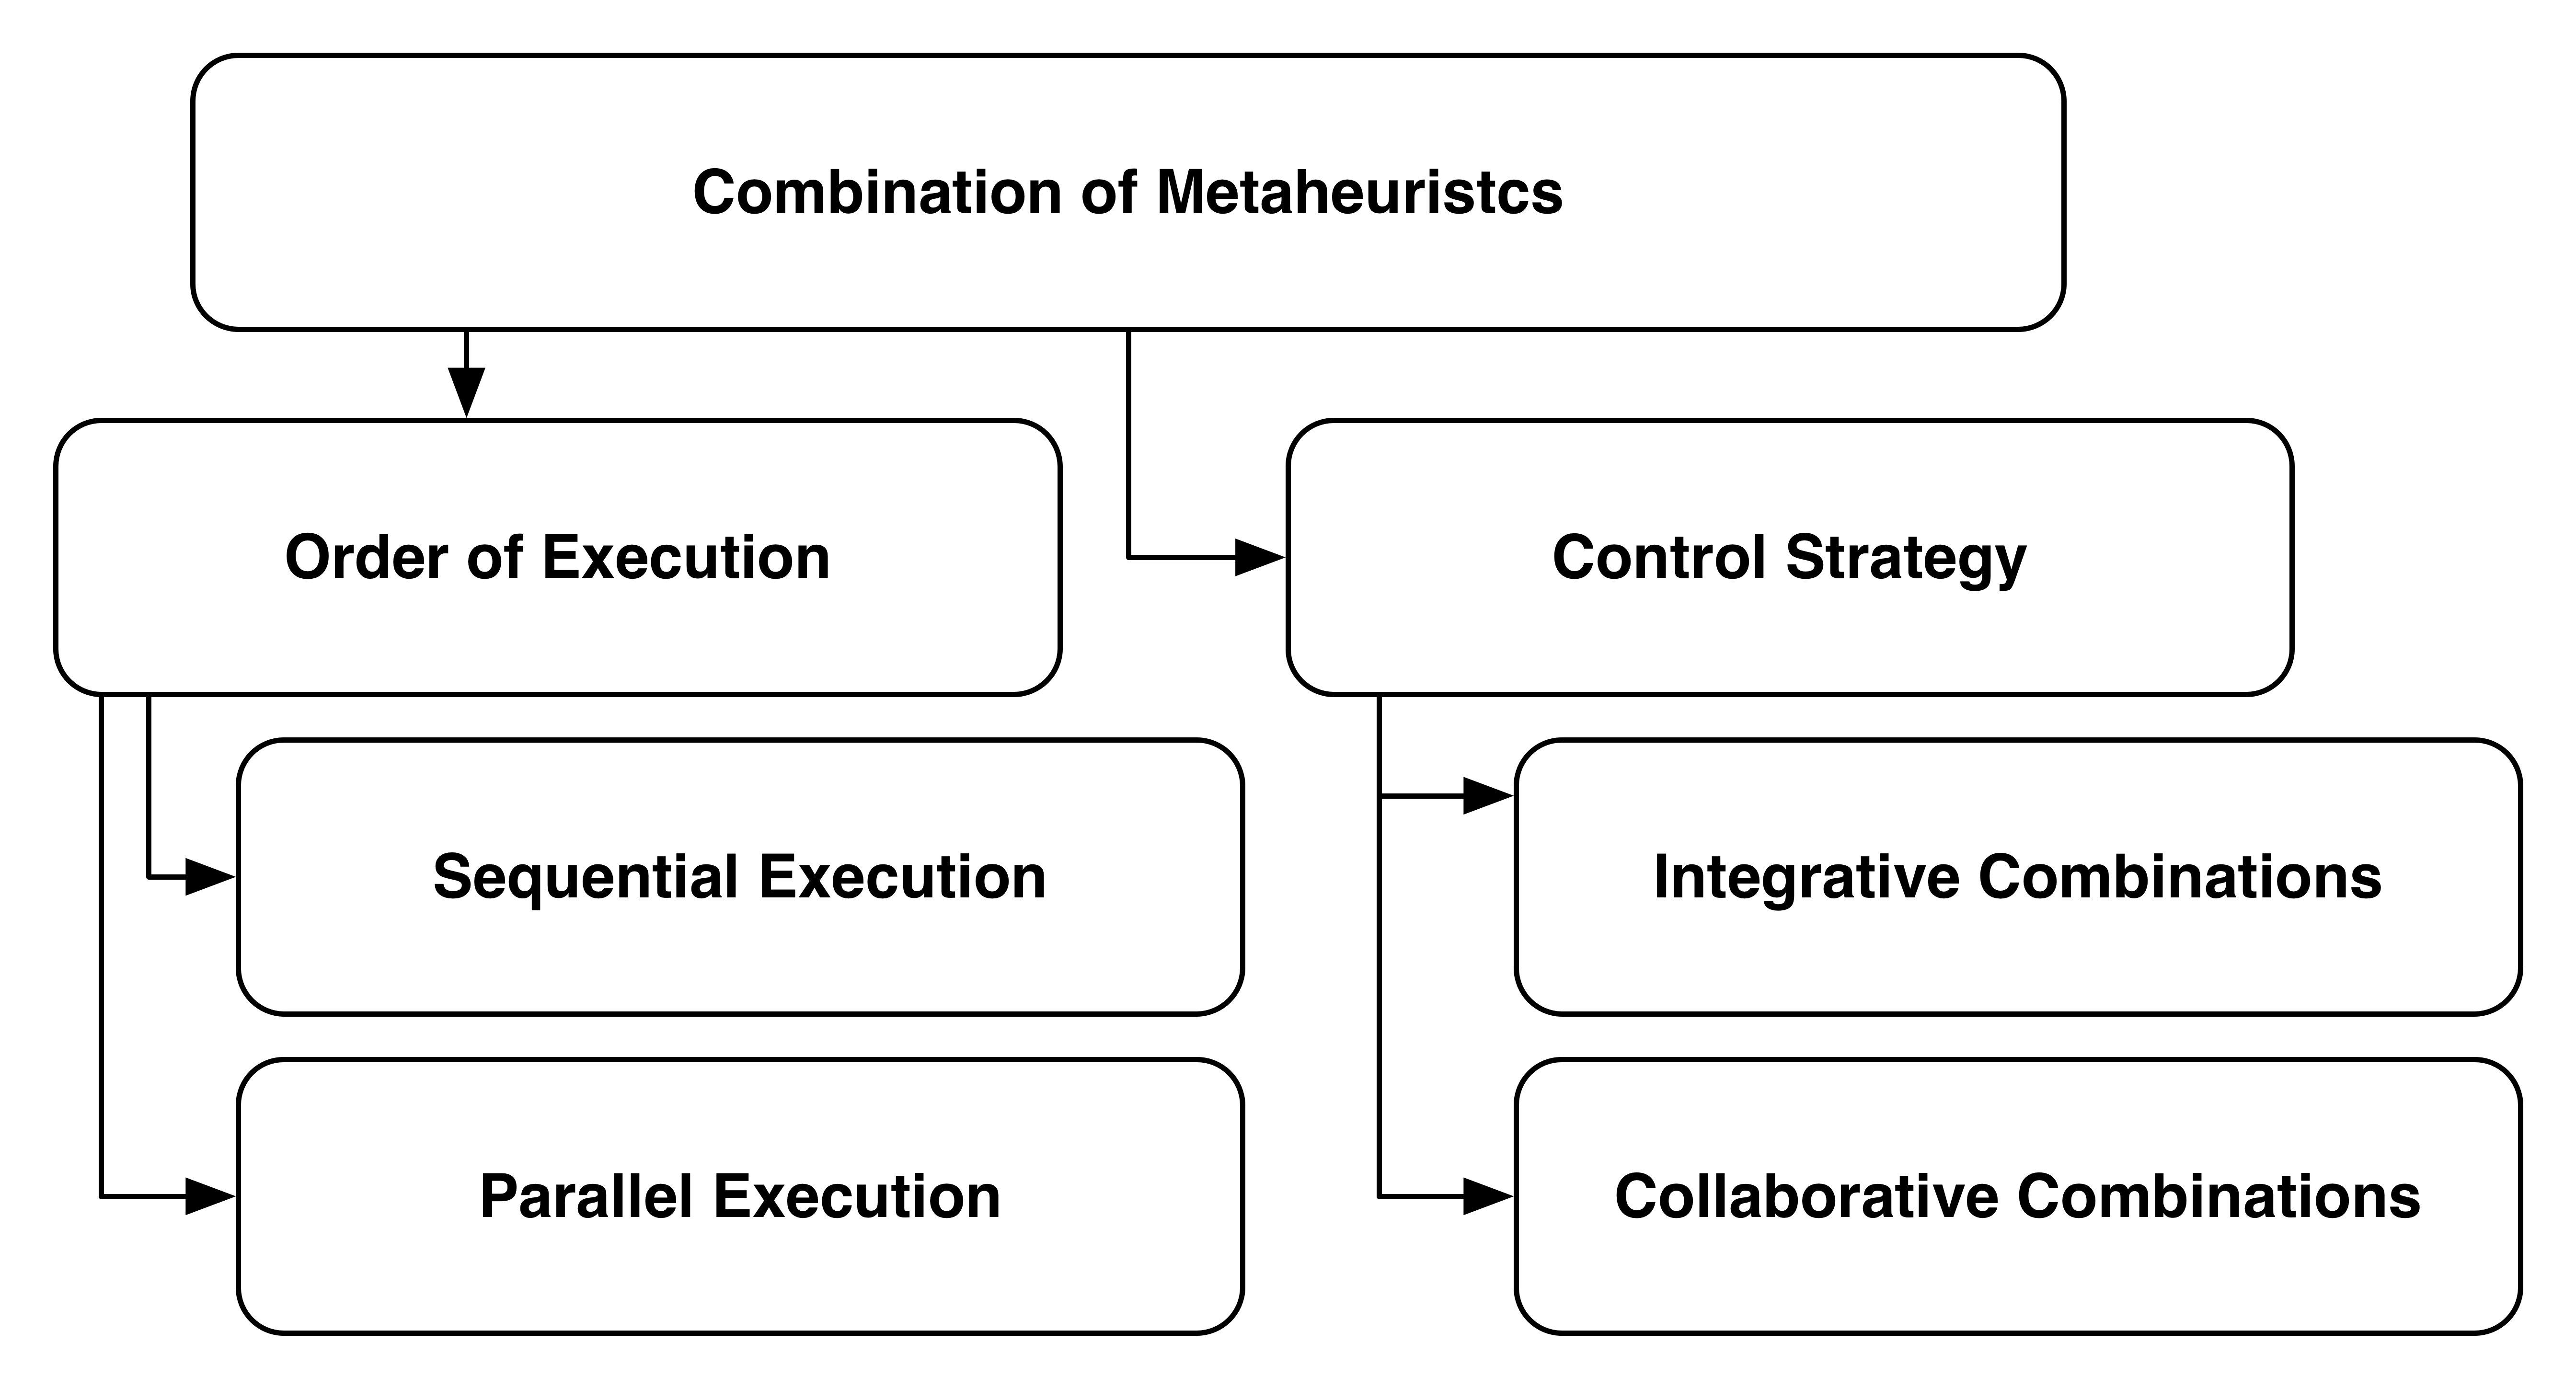
\includegraphics[width=0.5\textwidth]{./images/metaheuristc2.png}
\caption{Categories of metaheuristc combinations \cite{Puchinger2005} }
\label{fig:metaheuristc}
\end{figure}

Collaborative combinations use an approach where the algorithms exchange information, but are not part of each other. In this approach, algorithms may be executed sequentially or in parallel. 

One of the most popular ways of metaheuristic hybridization consists in the use of trajectory methods inside population-based methods. Population-based methods are better in identifying promising areas in the search space from which trajectory methods can quickly reach good local optima. Therefore, metaheuristic hybrids that can effectively combine the strengths of both population-based methods and trajectory methods are often very successful \cite{raidl2010metaheuristic}.


The work uses a type of collaborative combination with sequential execution with two trajectory methods (Tabu Search and Simulated Annealing) and Genetic Algorithms.

\section{Related Work}


The search for the longest execution time is regarded as a discontinuous, nonlinear, optimization problem, with the input domain of the system under test as a search space \cite{Sullivan}. 

A common goal of search-based stress testing is to find test scenarios that produce execution times that exceed the timing constraints specified. If a temporal error is found, the test was successful \cite{Sullivan}. The application of evolutionary algorithms to  stress tests involves finding the best- and worst-case execution times (B/WCET) to determine whether timing constraints are fulfilled \cite{Afzal2009a}. 


There are two measurement units normally associated with the fitness function in stress test: processor cycles and execution time. The processor cycle approach describes a fitness function in terms of processor cycles. The execution time approach involves executing the application under test and measuring the execution time \cite{Afzal2009a} \cite{tracey2000search}.

Processor cycles measurement is deterministic in the sense that it is independent of system load and results in the same execution times for the same set of input parameters. However, such a measurement is dependent on the compiler and optimizer used, therefore, the processor cycles differ for each platform. Execution time measurement is a non deterministic approach, there is no guarantee to get the same results for the same test inputs \cite{Afzal2009a}.  However, stress testing where testers have no access to the production environment should be measured by the execution time measurement \cite{Molyneaux2009} \cite{Afzal2009a}.

Table \ref{tab:comparison}  shows a comparison between the presented research work and the research studies on load, performance, and stress tests presented by Afzal et al. \cite{Afzal2009}. Afzal's work adds to some of the latest research in this area (\cite{Garousi2006} \cite{Garousi2010} \cite{DiAlesio2013} \cite{DiAlesio2014} \cite{Alesio2015}). 


The columns represent the type of tool used (prototype or functional tool), and the rows represent the metaheuristic approach used by each research study (genetic algorithm, Tabu search, simulated annealing, or a customized algorithm). The table also sorts the research studies by the type of fitness function used (execution time or processor cycles). Most research studies are limited to making prototypes of genetic algorithms. The presented research work is distinguished from others by having a functional tool using a hybrid approach. 


\begin{table}[h]
\centering
\caption{Distribution of the research studies over the range of applied metaheuristics}
\label{tab:comparison}
\begin{tabular}{p{1.2cm}|p{1.8cm}|p{1.8cm}|p{1.8cm}|}
\cline{2-4}
                                                                & \multicolumn{2}{c|}{\textbf{Prototypes}}            & \textbf{Functional Tool} \\ \cline{2-4} 
                                                                & \begin{minipage}{0.2\textwidth}\footnotesize Execution Time  \end{minipage}          & \begin{minipage}{0.2\textwidth}\footnotesize Processor Cycles \end{minipage}        & \begin{minipage}{0.2\textwidth}\footnotesize Execution Time \end{minipage}           \\ \cline{2-4} 
%\setlength{\extrarowheight}{20pt}
\begin{tabular}[c]{@{}l@{}}\begin{minipage}{0.1\textwidth}\scriptsize GA + SA  \\ + Tabu \\ Search \end{minipage}\end{tabular}  & \cellcolor[HTML]{FFFFFF} & \cellcolor[HTML]{FFFFFF} & \cellcolor[HTML]{F8FF00} \begin{minipage}{0.2\textwidth} \tiny \textbf{  \\ IADAPTER \\} \end{minipage}  \\[2ex] \cline{2-4} 
\begin{minipage}{0.1\textwidth}\scriptsize GA \end{minipage}                                                              & \cellcolor[HTML]{FFFFFF} \begin{minipage}{0.12\textwidth}   \tiny \textnormal{ \\  Alander et al.,1998 \cite{Alander} \\ Wegener et al., 1996 and 1997 \cite{Wegener1997}\cite{J.WegenerK.GrimmM.GrochtmannH.Sthamer1996} \\  Sullivan et al., 1998 \cite{Sullivan} \\ Briand et al., 2005 \cite{Briand2005} \\ Canfora et al., 2005 \cite{Canfora}  \\ }\end{minipage} & \cellcolor[HTML]{FFFFFF} \begin{minipage}{0.12\textwidth} \tiny \textrm{  \\ Wegener and Grochtmann, 1998 \cite{Wegener1998} \\  Mueller et al., 1998 \cite{Mueller1998} \\ Puschner et al. \cite{Puschner1998} \\ Wegener et al., 2000 \cite{Stations} \\ Gro et al., 2000 \cite{Gross2000}  \\ }\end{minipage}& \cellcolor[HTML]{FFFFFF} \begin{minipage}{0.12\textwidth}   \tiny \textnormal{ \\  Di Penta, 2007 \cite{Penta2007} \\ Garoussi, 2006 \cite{Garousi2006} \\ Garousi, 2008 \cite{Garousi2008} \\ Garousi, 2010 \cite{Garousi2010} \\ } \end{minipage} \\[2ex] \cline{2-4} 
\begin{minipage}{0.1\textwidth}\scriptsize Simulated \\ Annealing \\ (SA) \end{minipage}                                                             & \cellcolor[HTML]{FFFFFF} & \cellcolor[HTML]{FFFFFF} & \cellcolor[HTML]{FFFFFF} \begin{minipage}{0.12\textwidth}   \tiny  Tracey, 1998 \cite{Tracey1998} \end{minipage} \\[2ex] \cline{2-4}
\begin{minipage}{0.1\textwidth}\scriptsize  Constraint \\ Programming \end{minipage}                                                             & \cellcolor[HTML]{FFFFFF} & \cellcolor[HTML]{FFFFFF} & \cellcolor[HTML]{FFFFFF} \begin{minipage}{0.12\textwidth}   \tiny  Alesio, 2014 \cite{DiAlesio2014} \\ Alesio, 2013 \cite{DiAlesio2013}  \end{minipage} \\[2ex] \cline{2-4} 
\begin{minipage}{0.1\textwidth}\scriptsize  GA +\\ Constraint \\ Programming \end{minipage}                                                             & \cellcolor[HTML]{FFFFFF} & \cellcolor[HTML]{FFFFFF} & \cellcolor[HTML]{FFFFFF} \begin{minipage}{0.12\textwidth}   \tiny  Alesio, 2015 \cite{Alesio2015} \end{minipage} \\[2ex] \cline{2-4} 
\setlength{\extrarowheight}{20pt}
\begin{tabular}[c]{@{}l@{}}
\begin{minipage}{0.1\textwidth}\scriptsize Customized \\ Algorithm \end{minipage}\end{tabular} & \cellcolor[HTML]{FFFFFF} & \cellcolor[HTML]{FFFFFF}  \begin{minipage}{0.12\textwidth}   \tiny  \textnormal{   \raggedleft Pohlheim, 1999 \cite{Pohlheim2005}  } \end{minipage} & \cellcolor[HTML]{FFFFFF} \\[4ex] \cline{2-4}
\end{tabular}
\end{table}


Wegener et al. \cite{Wegener1997} used genetic algorithms(GA) to search for input situations that produce very long or very short execution times. The fitness function used was the execution time of an individual measured in micro seconds \cite{Wegener1997}. Alander et al. \cite{Alander} performed experiments in a simulator environment to measure response time extremes of protection relay software using genetic algorithms. The fitness function used was the response time of the tested software. The results showed that GA generated more input cases with longer response times \cite{Alander}. 

Wegener and Grochtmann performed a  experimentation
to compare GA with random testing. The fitness function used was duration of execution measured in processor cycles.  The results showed that, with a large number of input parameters, GA obtained more extreme execution times with less or equal testing effort than random testing \cite{J.WegenerK.GrimmM.GrochtmannH.Sthamer1996} \cite{Wegener1998}. Gro et. al. \cite{Gross2000} presented a prediction model  which can be used to predict evolutionary testability. The research confirmed that there is a relationship between the complexity of a test object and the ability of a search algorithm to produce input parameters according to B/WCET \cite{Gross2000}. 

Tracey et al. \cite{Tracey1998} used simulated annealing (SA) to test four
simple programs. The results of the research presented that the use of SA was more effective with larger parameter space. The authors highlighted the need of a detailed comparison of various optimization techniques to explore WCET and BCET of the of the system under test \cite{Tracey1998}.

Pohlheim and Wegener used an extension of genetic algorithms with multiple sub-populations, each using a different search strategy. The duration of execution measured in processor cycles was taken as the fitness
function. The GA found longer execution times for all the given modules in comparison with systematic testing\cite{Pohlheim2005}.

Briand et al. \cite{Briand2005} used GA to find the sequence of arrival times of events for aperiodic tasks, which will cause the greatest delays in the execution of the target task. A prototype tool named real-time test tool (RTTT) was developed to facilitate the execution of runs of genetic algorithm. Two case studies were conducted and results illustrated that RTTT was a useful tool to stress a system under test \cite{Briand2005}.

Di Penta et al. \cite{Penta2007} used GA to create test data that violated QoS constraints causing SLA violations. The generated test data included combinations of inputs. The approach was applied to two case studies. The first case study was an audio processing workflow. The second case study, a service producing charts, applied the black-box approach with fitness calculated only on the basis of how close solutions violate QoS constraint. In case of audio workflow, the GA outperformed random search. For the second case study, use of black-box approach successfully violated the response time constraint, showing the violation of QoS constraints for a real service available on the Internet \cite{Penta2007}.

Garousi presented a stress test methodology aimed at increasing chances of discovering faults related to distributed traffic in distributed systems. The technique uses as input a specified UML 2.0 model of a system, augmented with timing information.The results indicate that the technique is significantly more effective at detecting distributed traffic-related faults when compared to standard test cases based on an operational profile \cite{Garousi2006}.

Alesio describe stress test case generation as a search problem over the space of task arrival times. The research search for worst case scenarios maximizing deadline misses where each scenario characterizes a test case. The paper combine two strategies, GA and Constraint Programming (CP). The results show that, in comparison with GA and CP in isolation, GA+CP achieves nearly the same effectiveness as CP and the same efficiency and solution diversity as GA, thus combining the advantages of the two strategies. Alesio concludes that a combined GA+CP approach to stress testing is more likely to scale to large and complex systems \cite{Alesio2015}.

The presented research work and Alesio's approach \cite{Alesio2015} use a hybrid approach with a functional tool. Table \ref{tab:alesiogois} presents the main differences between Alesio's and IAdapter's approaches. Whereas the present research uses an approach based on usage scenarios performing tests on an application installed in an available environment, Alesio uses sequence diagrams  to select for arrival time of tasks in systems from  safety-critical domains. 


\begin{table}[H]
\centering
\caption{Main differences between Alesio's \cite{Alesio2015} and IAdapter's approaches}
\label{tab:alesiogois}
\begin{tabular}{l|l|l|}
\cline{2-3}
                                                                                  & Alesio et al. \cite{Alesio2015}                                                                                                             & IAdapter                                                                                                                            \\ \hline
\multicolumn{1}{|l|}{Metaheuristcs}                                               & \begin{tabular}[c]{@{}l@{}}GA+ \\ Constraint Programming\end{tabular}                                                      & \begin{tabular}[c]{@{}l@{}}GA+SA+\\ Tabu Search\end{tabular}                                                                           \\ \hline
\multicolumn{1}{|l|}{Inputs}                                                      & \begin{tabular}[c]{@{}l@{}}Design Model (Time and \\ Concurrency\\  Information)\end{tabular}                              & \begin{tabular}[c]{@{}l@{}}Number of Users\\ Ramp-up\\ Test scenarios\end{tabular}                                                     \\ \hline
\multicolumn{1}{|l|}{\begin{tabular}[c]{@{}l@{}}Main\\ Objective\end{tabular}}    & \begin{tabular}[c]{@{}l@{}}Find task arrival times\\ of aperiodic tasks that\\  maximizing\\  deadline misses\end{tabular} & \begin{tabular}[c]{@{}l@{}}Find the number of\\  users, ramp-up and \\ test scenarios that\\ maximizing\\ deadline misses\end{tabular} \\ \hline
\multicolumn{1}{|l|}{\begin{tabular}[c]{@{}l@{}}Main \\ Application\end{tabular}} & \begin{tabular}[c]{@{}l@{}}Systems from \\ safety-critical \\ domains\end{tabular}                                         & \begin{tabular}[c]{@{}l@{}}Web and Mobile \\ applications\end{tabular}                                                                 \\ \hline
\end{tabular}
\end{table}


\section{Improving Stress Search-Based Testing Using a Hybrid Metaheuristic Approach}


A large number of researchers have recognized the advantages and huge potential of building hybrid metaheuristics. The main motivation for creating hybrid metaheuristics is to exploit the complementary character of different optimization strategies. In fact, choosing an adequate combination of algorithms can be the key to achieving top performance in solving many hard optimization problems \cite{Puchinger2005} \cite{Blum2012}.

The proposed solution makes it possible to create a model that evolves during the test. The proposed solution model uses genetic algorithms, tabu search, and simulated annealing in two different approaches. The study initially investigated the use of these three algorithms. Subsequently, the study will focus in others Population-based and single point search metaheuristics. The first approach uses the three algorithms independently, and the second approach uses the three algorithms collaboratively (hybrid metaheuristic approach).

In the first approach , the algorithms do not share their best individuals among themselves. Each algorithm evolves in a separate way (Fig. \ref{fig:firstaproach}). The second approach uses the algorithms in a collaborative mode (hybrid metaheuristic). In this approach, the three algorithms share their best individuals found (Fig. \ref{fig:secondapproach}).

\begin{figure}[h]
\centering
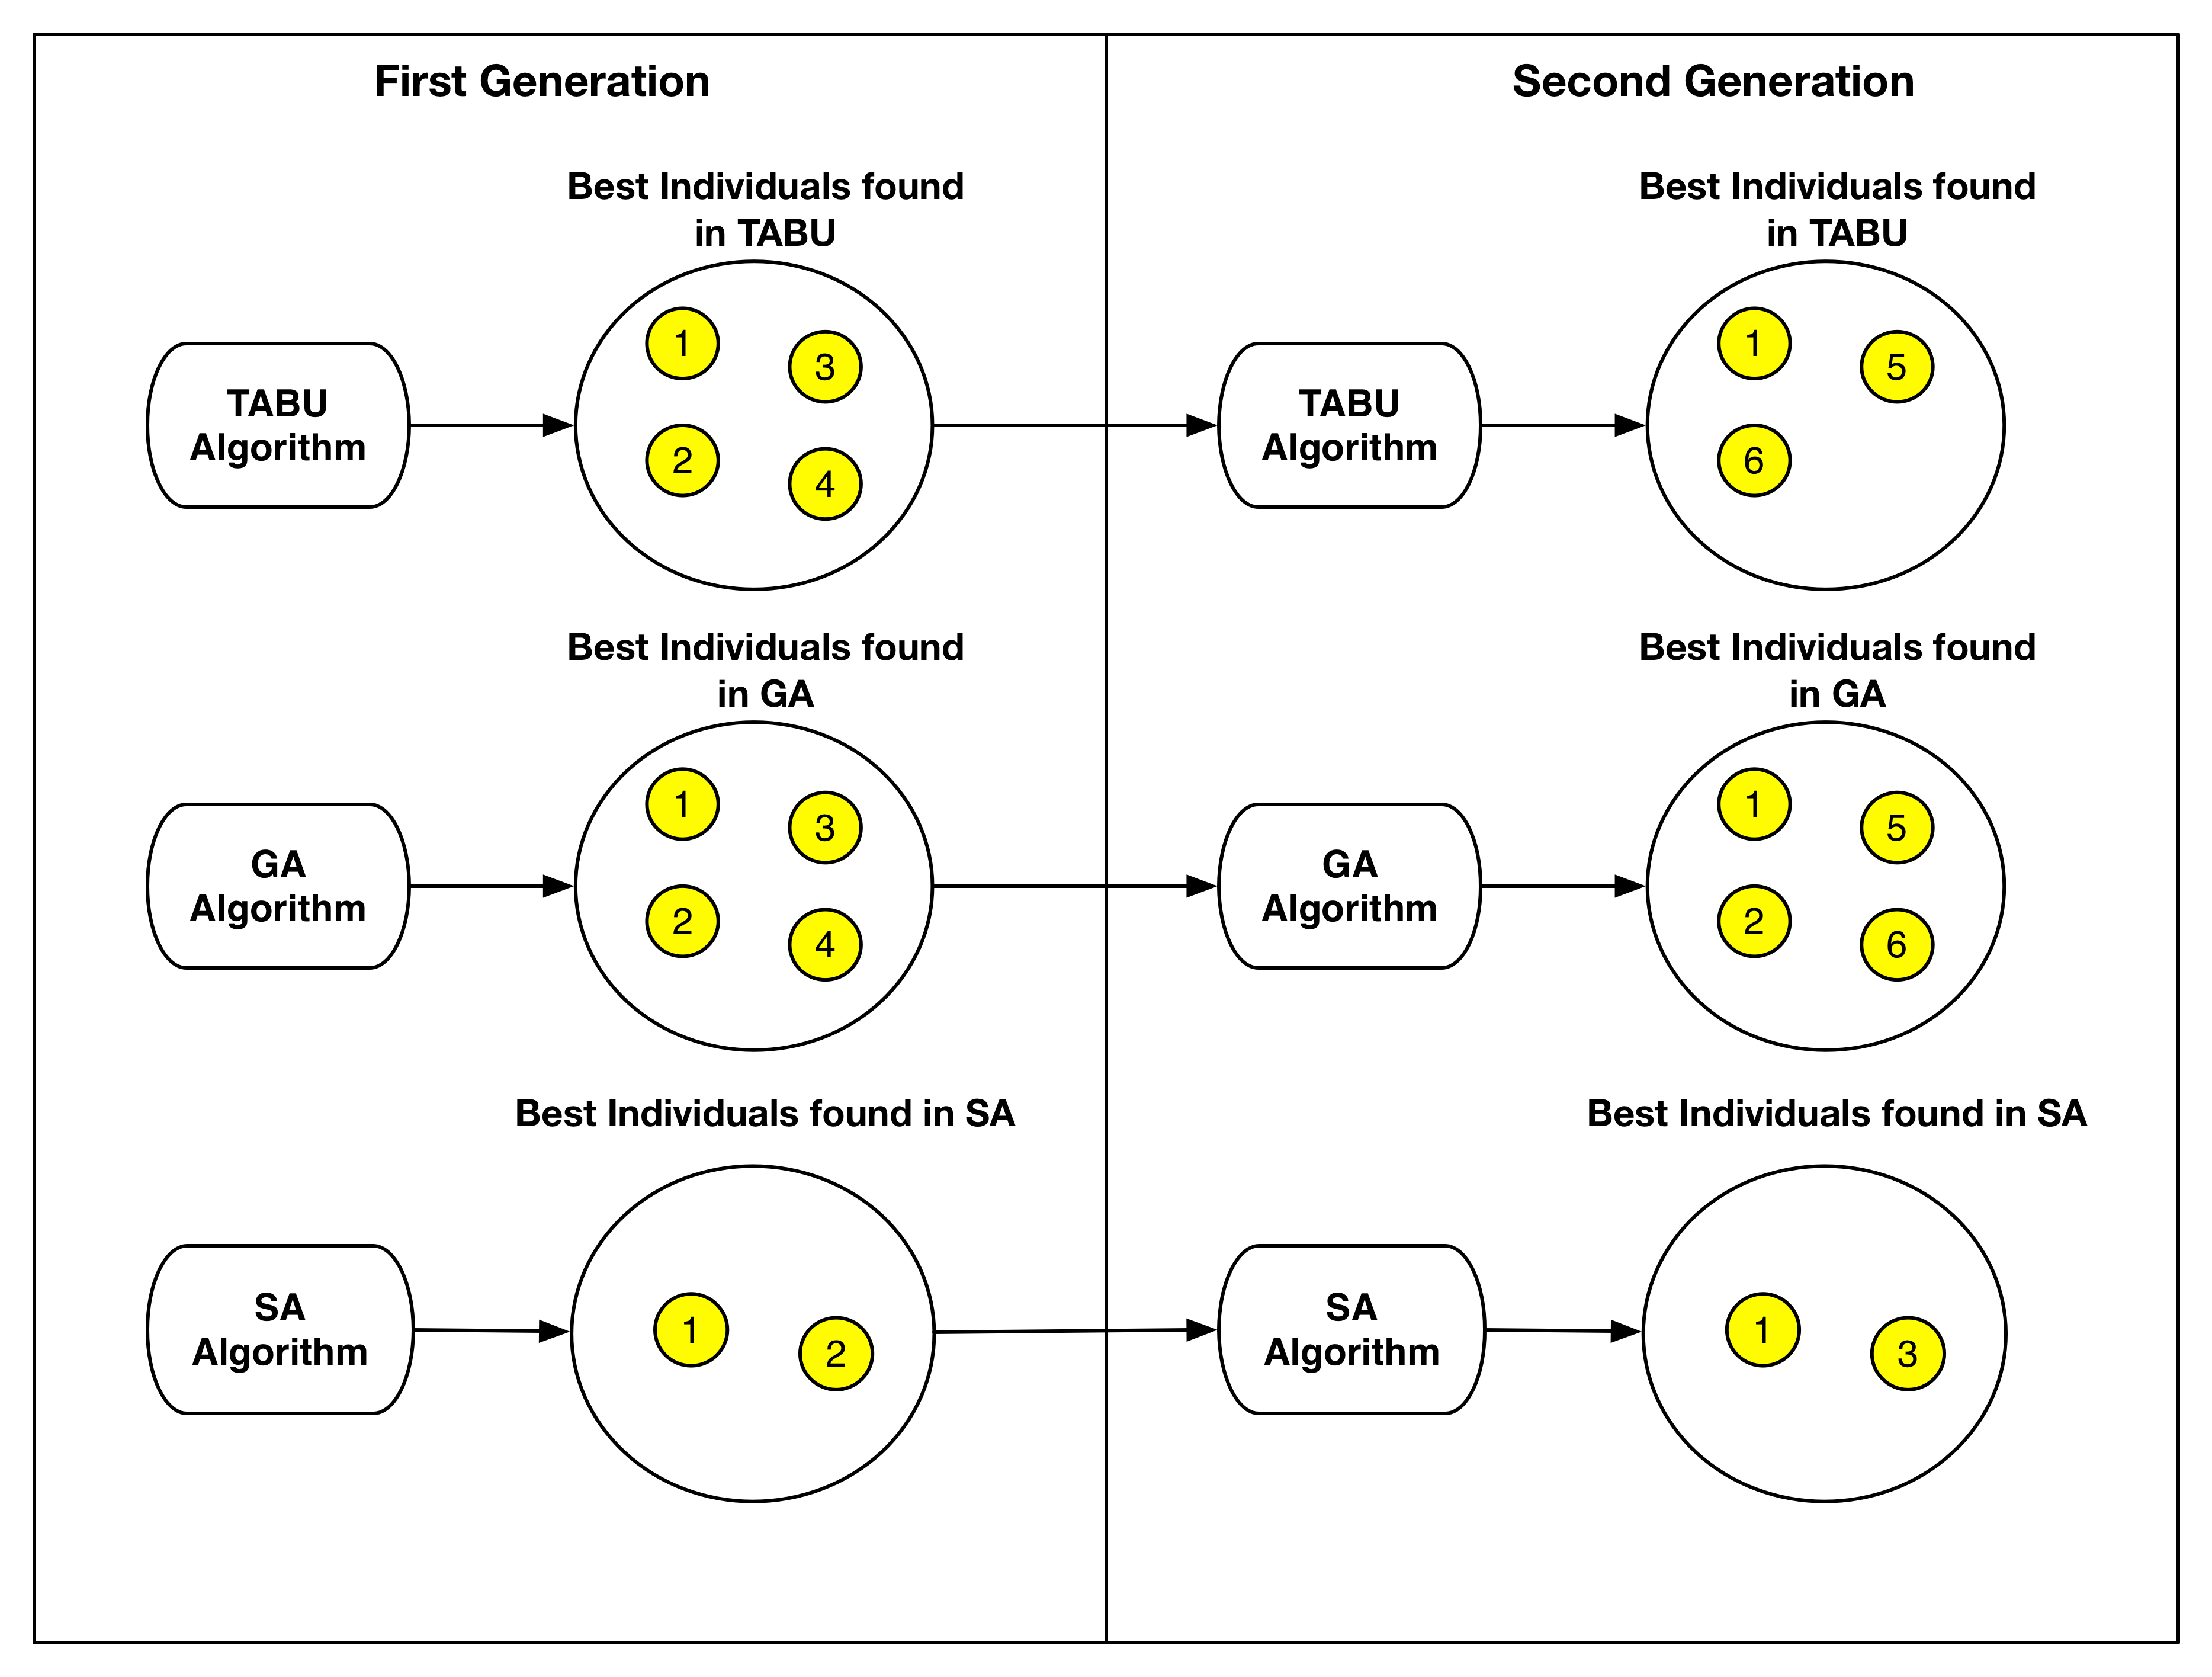
\includegraphics[width=0.5\textwidth]{./images/independ.png}
\caption{Use of the algorithms independently}
\label{fig:firstaproach}
\end{figure}

The next subsections present details about the used metaheuristic algorithms (Representation, initial population and fitness function).

\begin{figure}[h]
\centering
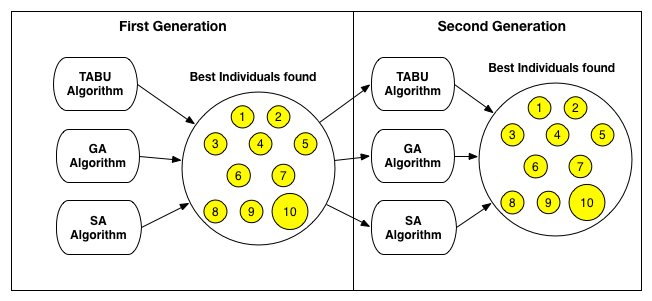
\includegraphics[width=0.5\textwidth]{./images/collaborative.png}
\caption{Use of the  algorithms collaboratively}
\label{fig:secondapproach}
\end{figure}

\subsection{Representation}

The solution representation is composed by a linear vector with 23 positions. The first position represents the name of an individual. The second position represents the algorithm (genetic algorithm, simulated annealing, or Tabu search) used by the individual. The third position represents the type of test (load, stress, or performance). The next positions represent 10 scenarios and their numbers of users. Each scenario is an atomic operation: the scenario must log into the application, run the task goal, and undo any changes performed, returning the application to its original state.

Fig. \ref{fig:genomarepresentation} presents the solution representation and an example using the crossover operation. In the example, genotype 1 has the Login scenario with 2 users, the Form scenario with 0 users, and the Search scenario with 3 users. Genotype 2 has the Delete scenario with 10 users, the Search scenario with 0 users, and the Include scenario with 5 users. After the crossover operation, we obtain a genotype with the Login scenario with 2 users, the Search scenario with 0 users, and the Include scenario with 5 users.

\begin{figure}[H]
\centering
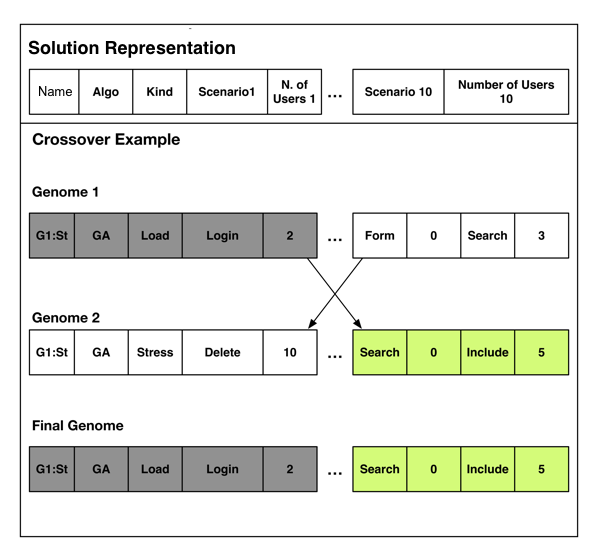
\includegraphics[width=0.5\textwidth]{./images/genomerepresentation1.png}
\caption{Solution representation and crossover example}
\label{fig:genomarepresentation}
\end{figure}

Fig. \ref{fig:neighbourtaby} shows the strategy used by the proposed solution to obtain the representation of the neighbors for the Tabu search and simulated annealing algorithms. The neighbors are obtained by the modification of a single position (scenario or number of users) in the vector.


\begin{figure}[H]
\centering
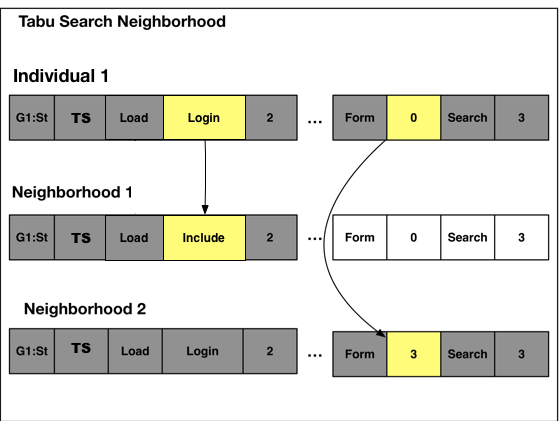
\includegraphics[width=0.5\textwidth]{./images/TabuNE2.png}
\caption{Tabu search and simulated annealing neighbor strategy}
\label{fig:neighbourtaby}
\end{figure}


\subsection{Initial population}

The strategy used by the plugin to instantiate the initial population is to generate 50\% of the individuals randomly, and 50\% of the initial population is distributed in three ranges of values:

\begin{itemize}
\item Thirty percent of the maximum allowed users in the test;
\item Sixty percent of the maximum allowed users in the test; and
\item Ninety percent of the maximum allowed users in the test.
\end{itemize}

The percentages relates to the distribution of the users in the initial test scenarios of the solution. For example, in a hypothetical test with 100 users, the solution will create initial test scenarios with 30, 60 and 90 users.

\subsection{Objective (fitness) function}

The proposed solution was designed to be used with independent testing teams in various situations where the teams have no direct access to the environment where the application under test was installed. Therefore, the IAdapter plugin uses a measurement approach to the definition of the fitness function. The fitness function applied to the IAdapter solution is governed by the following equation:

\begin{equation}
\begin{aligned}
fit=90percentileweigth* 90percentiletime\\
+80percentileweigth*80percentiletime\\+
70percentileweigth*70percentiletime+\\
maxResponseWeigth*maxResponseTime+\\
numberOfUsersWeigth*numberOfUsers-penalty
\end{aligned}
\end{equation}

The proposed solution's fitness function uses a series of manually adjustable user-defined weights (90percentileweight, 80percentileweight,  70percentileweight, maxResponseWeight, and numberOfUsersWeight). These weights make it possible to customize the search plugin's functionality. A penalty is applied when an application under test takes a longer time to respond than the level of service.


\FloatBarrier
\section{IAdapter}

IAdapter is a JMeter plugin designed to perform search-based stress tests.  The plugin is available on www.iadapter.org.  The IAdapter plugin implements the solution proposed in Section 5. The next subsections present details about the Apache JMeter tool, the IAdapter Life Cycle and the IAdapter Components. The IAdapter plugin provides three main components: WorkLoadThreadGroup, WorkLoadSaver, and WorkLoadController. The Fig. \ref{fig:iadapterarchitecture} show the IAdapter architecture. All metaheuristic class implements the interface IAlgorithm. Test scenarios  and test results are stored in a Mysql database. GeneticAlgorithm class uses a framework named JGAP to implement Genetic Algorithms.

\begin{figure}[H]
\centering
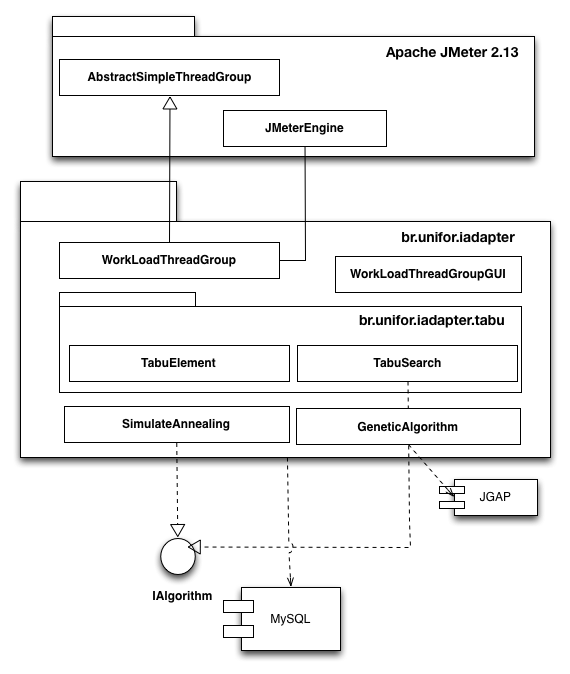
\includegraphics[width=0.5\textwidth]{./images/iadapter1.png}
\caption{IAdapter architecture}
\label{fig:iadapterarchitecture}
\end{figure}

The WorkLoadThreadGroup class is the Load Injection and Test Management modules, responsible to generate the initial population and uses the JMeter Engine to realize requests to server under test. 

\subsection{IAdapter Life Cycle}
 
Fig. \ref{fig:iadapterlifecycle} presents the IAdapter Life Cycle. The main difference between IAdapter and JMeter tool is that the IAdapter provide an automated test execution where the new test scenarios are choosen by the test tool.  In a test with JMeter, the tests scenarios are usually chosen by a test designer.

\begin{figure}[H]
\centering
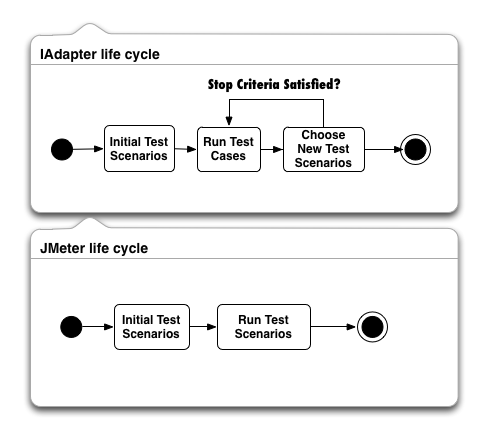
\includegraphics[width=0.6\textwidth]{./images/lifecycle2.png}
\caption{IAdapter life cycle}
\label{fig:iadapterlifecycle}
\end{figure}

\subsection{IAdapter Components}
 
WorkLoadThreadGroup is a component that creates an initial population and configures the algorithms used in IAdapter. Fig. \ref{fig:tela1iadapter} presents the main screen of the WorkLoadThreadGroup component. The component has a name \ding{202}, a set of configuration tabs \ding{203}, a list of individuals by generation \ding{204}, a button to generate an initial population \ding{205}, and a button to export the results \ding{206}.

\begin{figure}[H]
\centering
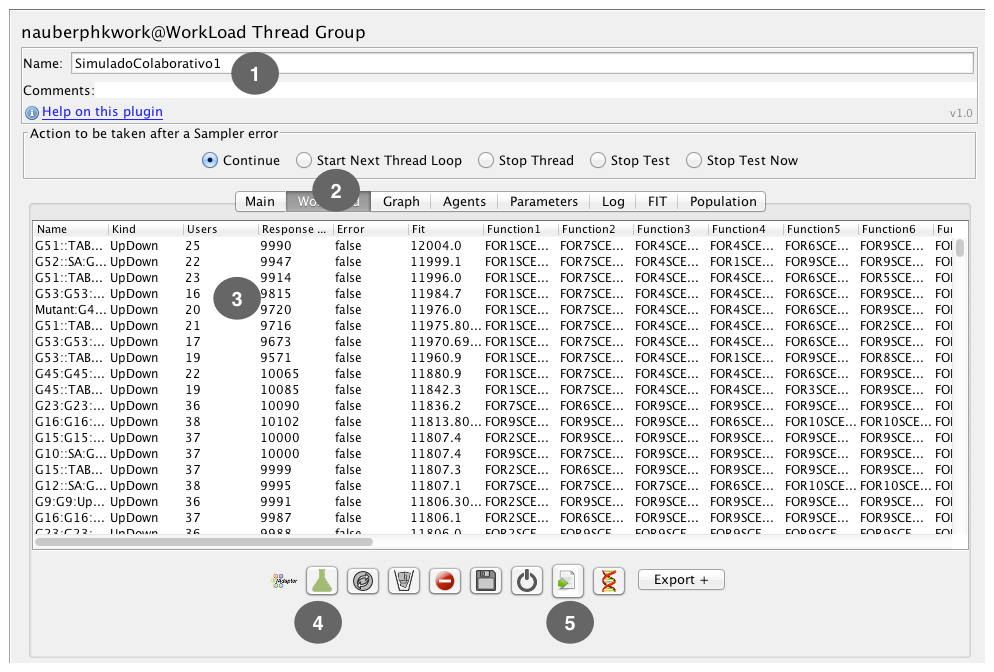
\includegraphics[width=0.9\textwidth]{./images/tela1iadapter.png}
\caption{WorkLoadThreadGroup component}
\label{fig:tela1iadapter}
\end{figure}

WorkLoadThreadGroup component uses the GeneticAlgorithm, TabuSearch and SimulateAnnealing classes. The Listing \ref{tabusearchclass} shows the Tabu Search class. The class has one main method named verify that remove all workload that are contained in the tabu list. The workloads are removed from tabu list when a expiration criteria it is satisfied.


\lstdefinestyle{outline}{
		language=Java,
         basicstyle=\scriptsize\ttfamily,
         numberstyle=\tiny,
         numbersep=5pt,
         tabsize=2,
         extendedchars=true,
         breaklines=true,
         keywordstyle=\color{black}\bf,
         frame=b,  % <<<<<<<<<<<<<<<<<<<<<<<<<<
         stringstyle=\color{green!40!black}\ttfamily,
         showspaces=false,
         showtabs=false,
         numbers=left,
         xleftmargin=17pt,
         framexleftmargin=17pt,
         framextopmargin=1pt, % <<<<<<<<<<<<<<<<<<<<<<
         showstringspaces=false,
         %backgroundcolor=\color[RGB]{200,200,200},
         belowcaptionskip=0pt
}



\begin{lstlisting}[style=outline,caption={TabuSearch class},label=tabusearchclass]
public class TabuSearch {

	private static int tabuExpires;

	private static List<TabuElement> tabuTable = new ArrayList<TabuElement>();

	public static List<WorkLoad> verify(List<WorkLoad> list, List<TestElement> nodes) {
	
	
	
		//ArrayList with the workloads to remove
		List<WorkLoad> workLoadForRemove = new ArrayList<WorkLoad>();
		for (WorkLoad workLoad : list) {
		    //Add elements in the tabu list to remotion
			for (TabuElement tabuElement : tabuTable) {
				TabuElement tabu = WorkLoadUtil.convertTabu(workLoad, nodes);
				workLoadForRemove.add(workLoad);			}
		}
		
		
		TabuSearch.setTabuExpires(TabuSearch.getTabuExpires() + 1);
		if (TabuSearch.getTabuExpires() > expiresCriteria)     
		{
		
			TabuSearch.setTabuTable(new ArrayList<TabuElement>());
			TabuSearch.setTabuExpires(0);
			
		}
		list.removeAll(workLoadForRemove);
		return list;
	}
\end{lstlisting}

The Listing \ref{saclass} shows the Simulated Annealing implementation. The algorithm iterate over a set of new places and accept new solutions with a better fitness value. Each new place represents a new workload in the stress test.


\begin{lstlisting}[style=outline,caption={Simulated Annealing Implementation},label=saclass]
//Simulated Annealing Method
public static int sa(int users, List<WorkLoad> newPlaces, int maxUsers,
			List<WorkLoad> list, int generation, WorkLoadThreadGroup tg,
			List<TestElement> nodes) {
		//Set Initial Temperature
		int newUsers = users;
		//Iterate in new places
		for (WorkLoad newPlace : newPlaces) {

			WorkLoad place = tg.getWorkloadCurrentSA();
			if (users > 0) {
				if ((place != null) && (newPlace != null)) {
					double deltaC = place.getFit() - newPlace.getFit();
					//If the new place has a better fitnesse value
					//Accept new solution
					if (deltaC < 0) {
						tg.setWorkloadCurrentSA(newPlace);

					} else {
					
						Random random = new Random();
						double randomDouble = random.nextDouble();
						SimulateAnnealing.tries += 1;
						double exponential = Math.exp(-1 * (deltaC / users));
						//Accept new solution with probability
						if (randomDouble > exponential) {
							tg.setWorkloadCurrentSA(newPlace);

						}
...
\end{lstlisting}


The WorkLoadSaver component is responsible for saving all data in the database. The operation of the component only requires its inclusion in the test script. WorkLoadController represents a scenario of the test. All actions necessary to test an application should be included in this component. All instances of the component need to login into the application under test and bring the application back to its original state.

\FloatBarrier
\section{Experiments}

This section presents two experiments. The first one was performed on an emulated component, and the second one was performed using an installed Moodle application. The experiments used the following fitness function:

\begin{equation}
\begin{aligned}
fit=0.9* 90percentiletime\\
+0.1*80percentiletime\\+
0.1*70percentiletime+\\
0.1*maxResponseTime+\\
0.2*numberOfUsers-penalty
\end{aligned}
\end{equation}

This fitness function is the same function represented in the section VII with the manually adjustable user-defined weights filled out. This fitness function intended to find individuals with the highest percentile of 90\%, followed by individuals with a higher percentile time of 80\% and 70\%, maximum response time, and number of users.

The first experiment ran for 27 generations, and the second experiment  performed 6 generations, with 300 executions by generation (100 times for each algorithm),  generating 300 new individuals. The experiments used an initial population of 100 individuals. The genetic algorithm used the top 10 individuals from each generation in the crossover operation. The Tabu list was configured with the size of 10 individuals and expired every 2 generations.  The mutation operation was applied to 10\% of the population on each generation. 

\subsection{First Experiment: Emulated Class Test}

The first experiment aimed to perform performance, load, and stress testing on a simulated component. The purpose of using a simulated component was to be able to perform a greater number of generations in a shorter time available and eliminate variables such as the use of databases and application servers. The first experiment used a test class  named SimulateConcurrentAccess. This class has a static variable named \textit{x} and a set of methods that use the variable in a synchronized context ( Listing \ref{classsimulated}). The experiment was executed using the JMeter Java Request Sampler Component with IAdapter.

\lstdefinestyle{outline}{
		language=Java,
         basicstyle=\scriptsize\ttfamily,
         numberstyle=\tiny,
         numbersep=5pt,
         tabsize=2,
         extendedchars=true,
         breaklines=true,
         keywordstyle=\color{black}\bf,
         frame=b,  % <<<<<<<<<<<<<<<<<<<<<<<<<<
         stringstyle=\color{green!40!black}\ttfamily,
         showspaces=false,
         showtabs=false,
         numbers=left,
         xleftmargin=17pt,
         framexleftmargin=17pt,
         framextopmargin=1pt, % <<<<<<<<<<<<<<<<<<<<<<
         showstringspaces=false,
         %backgroundcolor=\color[RGB]{200,200,200},
         belowcaptionskip=0pt
}

\begin{lstlisting}[style=outline,caption={SimulateConcurrentAccess class},label=classsimulated]
public class SimulateConcurrentAccess {
  @Test
  public void firstScenario() {		
    synchronized (StaticClass.class) {
			for (int i = 0; i <= 1000; i++) {
				StaticClass.x += i;
			}
			StaticClass.x = 0;
		}
	}
	
	  @Test
  public void secondScenario() {		
    synchronized (StaticClass.class) {
			for (int i = 0; i <= 2000; i++) {
				StaticClass.x += i;
			}
			StaticClass.x = 0;
		}
	}
\end{lstlisting}


Fig.\ref{fig:exp1bestresults} presents the best results in 27 generations applied in the first experiment. The figure shows the results obtained with the algorithms with and without collaboration. The $x$ axis  represents the generation number, and the $y$ axis represents the best fitness value obtained until the current generation.
A higher value in the figure means that the scenario has a greater response time by the application under test. The results of the experiment showed that the use of cooperation between the three algorithms resulted in finding the individuals with better fitness values.

\begin{figure}[H]
\centering
\caption{Best results obtained in 27 generations}
\includegraphics[width=1\textwidth]{./images/generationcomparative.png}
\label{fig:exp1bestresults}
\end{figure}

Table \ref{tab:averagefirst} presents the results obtained by the hybrid metaheuristic (HM) approach, genetic algorithm (GA), simulated annealing (SA), and Tabu search (TS) from 27 generations in the first experiment. The values are the maximum fitness value obtained by each algorithm. 

\begin{table}[H]
\centering
\caption{Maximum value of the fitness function by algorithm}
\label{tab:averagefirst}
\begin{tabular}{|l|l|l|l|l||l|l|l|l|l|}
\hline
GEN & HM & TS  & GA    & SA & GEN & HM & TS  & GA    & SA   \\ \hline
1          & 11238 & 11238         & 11238 & 11238 &  2          & 11804 & 11596         & 11801 & 10677 \\ \hline
3          & 11787 & 8932          & 8411  & 10869 &  4          & 11723 & 9753          & 9611  & 10760 \\ \hline
5          & 8164  & 9780          & 10738 & 4794  &  6          & 11802 & 9781          & 11086 & 6120  \\ \hline
7          & 9985  & 5782          & 11272 & 11798 &  8          & 11803 & 11749         & 10084 & 11309 \\ \hline
9          & 11806 & 7284          & 11633 & 10766 & 10         & 11807 & 9386          & 11717 & 4557  \\ \hline
11         & 11802 & 9653          & 11802 & 11151 & 12         & 11807 & 10594         & 11793 & 9434  \\ \hline
13         & 11802 & 10848         & 10382 & 11805 & 14         & 11801 & 11551         & 7219  & 10237 \\ \hline
15         & 11807 & 1701          & 7189  & 9338  & 16         & 11813 & 6203          & 11758 & 5321  \\ \hline
17         & 11805 & 10720         & 10805 & 11748 & 18         & 9600  & 6371          & 11698 & 7818  \\ \hline
19         & 11733 & 8160          & 11648 & 11509 & 20         & 9589  & 9428          & 11805 & 4813  \\ \hline
21         & 11800 & 9463          & 11798 & 10801 & 22         & 11805 & 11799         & 11804 & 6029  \\ \hline
23         & 11836 & 11655         & 11800 & 3579  & 24         & 11805 & 11512         & 11803 & 5761  \\ \hline
25         & 11804 & 11573         & 11802 & 9680  & 26         & 11800 & 11575         & 11403 & 9388  \\ \hline
27         & 11805 & 10691         & 11745 & 9465  & -          & -     & -             & -     & -      \\ \hline

\end{tabular}
\end{table}


The signed-rank Wilcoxon non-parametrical procedure was used for comparing the results with Z-value and W-value. The significant level adopted was 0.05. The Z-value obtained was -2.2736 and the p-value was 0.0232. The W-value obtained was 78. The critical value of W for N = 25 at p $\leq$ 0.05 was 89.The result was significant at p $\leq$ 0.05. The procedure showed that there was a significant improvement in the results with the collaborative approach.

\subsection{Second Experiment: Moodle Application Test}

The second experiment used a Moodle application installed in a machine with 500 GB of hard disk space and 8 GB of memory. The study used six application scenarios:

\begin{itemize}
\item PostDeleteMessage: This scenario posts and deletes messages in the Moodle application.
\item MyHome: This scenario accesses the homepage of the user's application.
\item Login: This scenario is responsible for user authentication by the application.
\item Notifications: This scenario involves entering the notification page of each user.
\item Start Page: This scenario shows the initial start page of the application.
\item Badge: This scenario involves entering the badge page.
\end{itemize}

The maximum tolerated response time in the test was 30 seconds.  Any  individuals who obtained a time longer than the stipulated maximum time suffered penalties.  The whole process of stress and performance tests, which took 3 days and about 1800 executions, was carried out without the need for monitoring by a test designer. The tool automatically selected the next scenarios to be run up to the limit of six generations previously established. 

Table \ref{tab:secondexperiment} presents the maximum fitness value obtained by the hybrid metaheuristic (HM) approach, genetic algorithm (GA), simulated annealing (SA), and Tabu search (TS) in each generation. 


\begin{table}[H]
\centering
\caption{Results obtained from the second experiment}
\label{tab:secondexperiment}
\begin{tabular}{|l|l|l|l|l|}
\hline
GEN & HM    & TS    & GA    & SA    \\
\hline
1          & 32242 & 32242 & 32242 & 32242 \\
\hline
2          & 34599 & 32443 & 26290 & 35635 \\
\hline
3          & 35800 & 34896 & 34584 & 34248 \\
\hline
4          & 35782 & 34912 & 32689 & 25753 \\
\hline
5          & 35611 & 31833 & 34631 & 8366  \\
\hline
6          & 35362 & 35041 & 33397 & 9706 \\
\hline
\end{tabular}
\end{table}


The small number of samples of the experiment is insufficient to give a statistical significance to the results of the Wilcoxon procedure. However, it is noted that, in four of six generations, the collaborative approach presented the best values. The experiment succeeded in finding 29 individuals whose maximum time expected by the application was obtained.  Table \ref{tab:secondexperiment1} shows an example of the six individuals with the highest fitness values in the second experiment. The table shows the fitness value (Fit);  the name of the scenario (Scenario); the number of users (Users); and the percentiles of 90\%, 80\%, and 70\% (90per, 80per and 70per) in seconds.  

% Please add the following required packages to your document preamble:
% \usepackage{multirow}
\begin{table}[h]
\centering
\caption{Example of individuals obtained in the second experiment}
\label{tab:secondexperiment1}
\begin{tabular}{|p{0.2cm}|l|l|l|p{0.60cm}|p{0.60cm}|p{0.60cm}|}
\hline
Id&Fit&Scenario&Users&90per&80per&70per\\ \hline
\multirow{2}{*}{1} & \multirow{2}{*}{35800} & MyHome        & 31              & \multirow{2}{*}{30} & \multirow{2}{*}{29} & \multirow{2}{*}{10} \\ \cline{3-4}
                   &                        & Badges        & 4               &                     &                     &                     \\ \hline
\multirow{3}{*}{2} & \multirow{3}{*}{35795} & MyHome        & 30              & \multirow{3}{*}{30} & \multirow{3}{*}{29} & \multirow{3}{*}{10} \\ \cline{3-4}
                   &                        & Notifications & 2               &                     &                     &                     \\ \cline{3-4}
                   &                        & Badges        & 2               &                     &                     &                     \\ \hline
\multirow{2}{*}{3} & \multirow{2}{*}{35782} & MyHome        & 32              & \multirow{2}{*}{30} & \multirow{2}{*}{29} & \multirow{2}{*}{10} \\ \cline{3-4}
                   &                        & Badges        & 3               &                     &                     &                     \\ \hline
\multirow{3}{*}{4} & \multirow{3}{*}{35773} & MyHome        & 22              & \multirow{3}{*}{30} & \multirow{3}{*}{29} & \multirow{3}{*}{10} \\ \cline{3-4}
                   &                        & Notifications & 6               &                     &                     &                     \\ \cline{3-4}
                   &                        & Badges        & 9               &                     &                     &                     \\ \hline
\multirow{2}{*}{5} & \multirow{2}{*}{35771} & MyHome        & 28              & \multirow{2}{*}{30} & \multirow{2}{*}{29} & \multirow{2}{*}{9}  \\ \cline{3-4}
                   &                        & Badges        & 6               &                     &                     &                     \\ \hline
\multirow{2}{*}{6} & \multirow{2}{*}{35683} & MyHome        & 27              & \multirow{2}{*}{30} & \multirow{2}{*}{29} & \multirow{2}{*}{8}  \\ \cline{3-4}
                   &                        & Badges        & 10              &                     &                     &                     \\ \hline
\end{tabular}
\end{table}


Table \ref{fig:gened} presents the percentage of genes in all test scenarios by generation with and without collaboration. Most of the genes converged to the MyHome feature, which had the highest application response time.


% Please add the following required packages to your document preamble:
% \usepackage[table,xcdraw]{xcolor}
% If you use beamer only pass "xcolor=table" option, i.e. \documentclass[xcolor=table]{beamer}
\begin{table}[H]
\centering
\caption{Percentage of genes in each scenario by generation }
\label{fig:gened}
\begin{tabular}{c|c|c|c|c|c|c|c|}
\hline
\rowcolor[HTML]{D3D3D3} 
\multicolumn{1}{|c|}{\cellcolor[HTML]{FFFFFF}\textbf{Gen/}}   & \multicolumn{7}{c|}{\cellcolor[HTML]{D3D3D3}\textbf{Non collaboration approach}}                                                                                                                                                       \\ \cline{2-8} 
\multicolumn{1}{|c|}{\textbf{Scenarios}}                      & \cellcolor[HTML]{F8FF00}Initial & \cellcolor[HTML]{F8FF00}1 & \cellcolor[HTML]{F8FF00}2 & \cellcolor[HTML]{F8FF00}3 & \cellcolor[HTML]{F8FF00}4 & \cellcolor[HTML]{F8FF00}5 & \cellcolor[HTML]{F8FF00}6                                \\ \hline
\multicolumn{1}{|c|}{\cellcolor[HTML]{D3D3D3}Badges}          & 20                              & 18                        & 16                        & 24                        & 15                        & 16                        & 17                                                       \\ \hline
\rowcolor[HTML]{F8FF00} 
\multicolumn{1}{|c|}{\cellcolor[HTML]{F8FF00}\textbf{MyHome}} & \textbf{15}                     & \textbf{59}               & \textbf{55}               & \textbf{48}               & \textbf{53}               & \textbf{50}               & \multicolumn{1}{l|}{\cellcolor[HTML]{F8FF00}\textbf{52}} \\ \hline
\multicolumn{1}{|c|}{\cellcolor[HTML]{D3D3D3}StartPage}       & 15                              & 10                        & 12                        & 11                        & 20                        & 18                        & \multicolumn{1}{l|}{19}                                  \\ \hline
\multicolumn{1}{|c|}{\cellcolor[HTML]{D3D3D3}Notifications}   & 25                              & 5                         & 11                        & 10                        & 9                         & 10                        & \multicolumn{1}{l|}{9}                                   \\ \hline
\multicolumn{1}{|c|}{\cellcolor[HTML]{D3D3D3}Post}            & 8                               & 3                         & 1                         & 3                         & 1                         & 2                         & \multicolumn{1}{l|}{1}                                   \\ \hline
\multicolumn{1}{|c|}{\cellcolor[HTML]{D3D3D3}Login}           & 17                              & 5                         & 5                         & 4                         & 2                         & 4                         & \multicolumn{1}{l|}{2}                                   \\ \hline
\multicolumn{1}{l|}{}                                         & \multicolumn{7}{c|}{\cellcolor[HTML]{D3D3D3}\textbf{Collaboration approach}}                                                                                                                                                           \\ \hline
\multicolumn{1}{|c|}{\cellcolor[HTML]{D3D3D3}Badges}          & 20                              & 29                        & 16                        & 25                        & 9                         & 16                        & 9                                                        \\ \hline
\rowcolor[HTML]{F8FF00} 
\multicolumn{1}{|c|}{\cellcolor[HTML]{F8FF00}\textbf{MyHome}} & \textbf{15}                     & \textbf{29}               & \textbf{69}               & \textbf{49}               & \textbf{74}               & \textbf{66}               & \textbf{76}                                              \\ \hline
\multicolumn{1}{|c|}{\cellcolor[HTML]{D3D3D3}StartPage}       & 15                              & 22                        & 10                        & 21                        & 10                        & 10                        & 8                                                        \\ \hline
\multicolumn{1}{|c|}{\cellcolor[HTML]{D3D3D3}Nofications}     & 25                              & 10                        & 1                         & 1                         & 2                         & 1                         & 3                                                        \\ \hline
\multicolumn{1}{|c|}{\cellcolor[HTML]{D3D3D3}Post}            & 8                               & 2                         & 1                         & 1                         & 1                         & 2                         & 1                                                        \\ \hline
\multicolumn{1}{|c|}{\cellcolor[HTML]{D3D3D3}Login}           & 17                              & 8                         & 3                         & 3                         & 4                         & 5                         & 3                                                        \\ \hline
\end{tabular}
\end{table}


%\begin{figure}[h]
%\centering
%\caption{Percentage of genes in all test scenarios by generation }
%\includegraphics[width=0.5\textwidth]{./images/gened.png}
%\label{fig:gened}
%\end{figure}

\FloatBarrier

\section{Conclusion}

This paper presented a hybrid metaheuristic approach for use in stress testing. Two experiments were performed to validate the solution. The first experiment was performed on an emulated component, and the second experiment was performed using an installed Moodle application.  The collaborative approach obtained better fit values in both experiments. The main contributions of this research are as follows: The presentation of a hybrid metaheuristic approach for use in stress tests; the development of a JMeter plugin  for search-based tests; and  the automation of the stress test execution process.  

In the first experiment, the signed-rank Wilcoxon non-parametrical procedure was used for comparing the results. The significant level adopted was 0.05. The procedure showed that there was a significant improvement in the results with the Hybrid Metaheuristic approach. In the second experiment, the whole process of stress and performance tests, which took 3 days and about 1800 executions, was carried out without the need for monitoring by a test designer. The tool automatically selected the next scenarios to be run up to the limit of six generations previously established. 

There is a range of future improvements in the proposed approach. Also as a typical search strategy, it is difficult to ensure that the execution times generated in the experiments represents global optimum. More experimentation is also required to determine the
most appropriate and robust parameters. Lastly, there is a need for an adequate termination criterion to stop the search process. Among the future works of the research, the use of new combinatorial optimization algorithms such as very large-scale neighborhood search is one that we can highlight


%\section*{Reference}

%% The Appendices part is started with the command \appendix;
%% appendix sections are then done as normal sections
%% \appendix

%% \section{}
%% \label{}

%% References
%%
%% Following citation commands can be used in the body text:
%% Usage of \cite is as follows:
%%   \cite{key}          ==>>  [#]
%%   \cite[chap. 2]{key} ==>>  [#, chap. 2]
%%   \citet{key}         ==>>  Author [#]

%% References with bibTeX database:


\bibliographystyle{IEEEtran}
\bibliography{sample}

\end{document}

